\documentclass{article}
\usepackage{times}
\usepackage{amssymb}
\usepackage{amsmath}
\usepackage{amsthm}
\usepackage{amsxtra}
\usepackage{algorithm}
\usepackage{algpseudocode}
\usepackage{color}
\usepackage{listings}
\usepackage{graphicx}

\newtheorem{theorem}{Theorem}

\newtheorem{myexample}{\textbf{Example}}
\newtheorem{mylemma}{\textbf{Lemma}}
\newtheorem{myproof}{\textbf{Proof}}
\newtheorem{myinvariant}{\textbf{Invariant}}
\newtheorem{mytheorem}{\textbf{Theorem}}
\newtheorem{mycorollary}{\textbf{Corollary}}
\newtheorem{myapproach}{Approach}
\newtheorem{myproperty}{Property}
\newtheorem{myproposition}{Proposition}
\newtheorem{mydefinition}{Definition}
\newtheorem{myassumption}{Assumption}

\newtheorem{mycase}{Case}

\lstset{ %
  backgroundcolor=\color{white},   % choose the background color; you must add \usepackage{color} or \usepackage{xcolor}
  basicstyle=\footnotesize,        % the size of the fonts that are used for the code
  breakatwhitespace=false,         % sets if automatic breaks should only happen at whitespace
  breaklines=true,                 % sets automatic line breaking
  captionpos=b,                    % sets the caption-position to bottom
  commentstyle=\color{mygreen},    % comment style
  deletekeywords={...},            % if you want to delete keywords from the given language
  escapeinside={\%*}{*)},          % if you want to add LaTeX within your code
  extendedchars=true,              % lets you use non-ASCII characters; for 8-bits encodings only, does not work with UTF-8
  frame=single,                    % adds a frame around the code
  keepspaces=true,                 % keeps spaces in text, useful for keeping indentation of code (possibly needs columns=flexible)
  keywordstyle=\color{blue},       % keyword style
  language=Octave,                 % the language of the code
  morekeywords={assign, repeat, then, increment, decrement, jump, jump_if, store, *, +},            % if you want to add more keywords to the set
  numbers=left,                    % where to put the line-numbers; possible values are (none, left, right)
  numbersep=5pt,                   % how far the line-numbers are from the code
  rulecolor=\color{black},         % if not set, the frame-color may be changed on line-breaks within not-black text (e.g. comments (green here))
  showspaces=false,                % show spaces everywhere adding particular underscores; it overrides 'showstringspaces'
  showstringspaces=false,          % underline spaces within strings only
  showtabs=false,                  % show tabs within strings adding particular underscores
  stepnumber=1,                    % the step between two line-numbers. If it's 1, each line will be numbered
  stringstyle=\color{red},     % string literal style
  tabsize=2,                       % sets default tabsize to 2 spaces
  title=\lstname                   % show the filename of files included with \lstinputlisting; also try caption instead of title
}


\title{Algorithms and Data Structures}

\begin{document}

\maketitle

%\section{Stable Matching}

Discussed by Gale, Shapley in 1962 (context of job markets): This problem is also related the allocation of workers in hospitals.

Each company a strict preference over applicants. Applicant has a strict preference over companies.

Is there a solution that is self-enforcing?

\begin{mydefinition}[Self-enforcing]
A matching is self-enforcing if for every applicant A and company C, such that A is not assigned to C, either:
\begin{itemize}
\item C prefers every one of its accepted applicants over A, or 
\item A prefers his current situation over working for C.
\end{itemize}
\end{mydefinition}



\section{Formal Model}

\begin{itemize}
\item Set X of man, 	$n = |X|$

\item Set Y of woman,	$m = |Y|$

\item Each $x \in X$ has a strict preference order $>_x$ over $Y$.

\item Each $y \in Y$ has a strict preference order $>_y$ over $X$.

\item Matching $M \subseteq X \times Y$ is a set of ordered pairs such that
every agent appears in at most one pair.
\end{itemize}

A blocking pair $(x,y)$ is a pair such that either $x$ or $y$ prefers some other person than its current match. A stable matching does not have blocking pairs.

\textbf{Problem:} Does there always exist a stable matching? Can we compute it in polynomial time?

Note: There may be solutions that are unfair, that is, they satisfy only one side (companies or workers).

\section{Deferred Acceptance Algorithm}

\textbf{Main idea}: Starts with an empty set of edges.

\begin{algorithmic}[1]
    \State{Initially, all $x \in X$ and all $y \in Y$ are free.}
    \While{$\exists$ free man $x$ that has not proposed to all women}
        \State{Let $y$ be the highest-ranked proposed women for $x$ that he hasn't proposed to
}
        \State{$x$ proposes to $y$}
        \If{$y$ is free}
            \State{$(x,y)$ gets engaged}
        \Else
            \State{$y$ currently engaged to $x'$}
            \If{$x >_y x'$}
                \State{$(x,y)$ gets engaged and $x'$ becomes free}
            \EndIf
        \EndIf
    \EndWhile
\end{algorithmic}

\begin{theorem}
The DA algorithm terminates after $n \cdot m$ iterations.
\end{theorem}
\begin{proof}
Some straightforward properties:
\begin{enumerate}
\item If $y$ becomes engaged, she will be matched in the end. The engagement partners are improving with respect to her preference $>_y$ over time.
\item $x$ proposes in decreasing order of $>_x$.
Thus, number of iterations is upper bounded by $n \cdot m$.
\end{enumerate}

Let $y >_x y'$ and $x >_y x'$. By contradiction, suppose in the final matching there is a BP, that is, we have a matching $M=\{(x,y'), (x', y)\}$.

- Note that $y >_x y'$, so by algorithm, $x$ proposed to $y$.

- Then $x$ proposed to $y'$, but $x$ becomes free afterwards.

- $y$ had a better engaged partner $x' >_y x$.

Contradiction.
\end{proof}

\subsection{Formalisms}

\begin{enumerate}

\item Woman $y$ is a \emph{valid partner} for a man $x$ if there exists a SM $M$ with $(x,y) \in M$.

\item Valid partner $y$ is the \emph{best valid partner} for man $x$ if for every valid partner $y' \neq y$, we have that $y >_x y'$.

\item Similar for \emph{worst valid partner}.
\end{enumerate}

\textbf{Notation:} $y = best(x)$ and $best(x) = x$ if $x$ has no valid partner.

We define the optimal matching as follows:

$$M^+ = \{ (x, best(x) | x \in X \wedge best(x) \neq x\}$$

\begin{theorem}
Every execution of the DA algorithm results in $M^+$.
\end{theorem}
\begin{proof}
Contradiction. Assume there is an execution $E$ of the DA algorithm resulting in a SM $M$, where some man is not matched to his best valid partner. This means that this man was rejected by a better valid partner during $E$.

Consider the first time that this happens, i.e., a man $x$ is rejected by a valid partner.

We have $(x',y)$, with $x' >_y x$.

\begin{enumerate}
\item $x$ proposed in decreasing order of preference, $y$ is ${best}(x)$.
\item $y$ rejects $x$, so $y$ is engaged to $x'$, with $x' >_y x$.
\item There exists Sm M with $(x,y) \in M$. Let $(x', y') \in M$.
\item Since rejection by $y$ was first in $E$, then $x'$ is not rejected by any valid partner when engaged to $y$. Since $y'$ is a valid partner of $x'$, $y >_x y'$. Then $(x', y)$ is a BP for $M$. But we assumed that $M$ is stable! Contradiction.
\end{enumerate}
\end{proof}

\begin{theorem}
In $M^+$, every woman is matched to her worst valid partner (if any).
\end{theorem}
\begin{proof}
Suppose $(x,y) \in M^+$ such that $x$ is not the worst valid partner of $y$.
Then there exists an SM $M'$ with $(x', y) \in M'$ and $x >_y x'$.
In $M'$ we have $(x, y') \in M'$. $y = {best}(x)$ and $y'$ is a valid partner for $x$. So $y >_x y'$. Then $(x,y)$ is a BP in $M'$. Contradiction.
Similar if $x$ is unmatched in $M'$.
\end{proof}

%\newpage

\section{Prerequisites}

\begin{itemize}

\item \textbf{Algorithm:} A step-by-step procedure for solving a certain \emph{problem}, e.g., ``sorting $n$ numbers'', ``find the closest coffee shop to your position''.

\item \textbf{Quality Criteria:} termination,  correctness, speed, memory, simplicity, generality, randomization, approximation Quality.

\item \textbf{Data Structure:} An organization of data such that certain operations can be handled efficiently. Ex: lists, heaps, etc.

\item \textbf{Quality Criteria:} memory, preprocessing time, query time, update time, simplicity

\end{itemize}

To evaluate the performance, we require a model.


\subsection{Random Access Model}

Memory consists of a sequence of cells, with an address ${addr} \in \mathbb{N}$. There are registers that can hold data, where operations may be performed. We assume the word size if polynomially bounded in $\log n$.

In this model, an algorithm is a numbered sequence of basic operations. The input of size $m$ for the algorithm is stored in memory $\{0, \ldots, m-1\}$. We have the following basic operations:

\begin{enumerate}
\item \textbf{load($i$, $j$):} Loads the content the memory cell with address stored in register $i$ into register $R_j$.
\item \textbf{store($i$, $j$):} Stores the content of register $i$ into the memory cell addressed by register $R_j$.
\item \textbf{assign($i$, $C$):} Stores $C$ into register $R_i$.
\item \textbf{increment/decrement($i$):} Increases/decreases value at $R_i$ by 1.
\item \textbf{op($i$, $j$, $k$):} Stores $R_i {op} R_j$ into $R_k$. ${op} \in \{+, \times, 0, \div, \mod, \wedge, \vee, \ldots\}$.
\item \textbf{jump($i$):} Jumps to operation $i$ in the algorithm.
\item \textbf{jump\_if($i$, $j$):} Jumps to operation $i$ in the algorithm if $R_j = 0$.
\end{enumerate}

\begin{algorithm}[h]
\begin{lstlisting}
assign(1, n) %*\quad*) -- 1
assign(2, 0) %*\quad*) -- 1
decrement(1) %*\quad*) -- n
load(1,3) %*\quad*) -- n
*(3,3,3) %*\quad*) -- n
+(3,2,2) %*\quad*) -- n
jump_if(8,1) %*\quad*) -- n
jump(2) %*\quad*) -- n-1
store(2,0) %*\quad*) -- 1
\end{lstlisting}
\caption{Add the squares of the first $n$ numbers in memory. The time complexity is $6n +2$.}
\end{algorithm}

\textbf{Cost Model}: Every basic operation takes one time unit to execute.

\begin{mydefinition}[Time Complexity]
The time complexity/runtime of algorithm $A$ for input $I$, $T_A(I)$, is the number of basic operations performed by $A$ on $I$.
\end{mydefinition}

With this definition of time complexity, we can compare speeds using natural functions.

\begin{mydefinition}[Worst-case]
The worst-case complexity $T_A^{wc}(n)$ of algorithm $A$ is equal to $\max\{I_A(I) | I \in I_n\}$.
\end{mydefinition}

\begin{mydefinition}[Best-case]
The best-case complexity $T_A^{wc}(n)$ of algorithm $A$ is equal to $\min\{I_A(I) | I \in I_n\}$.
\end{mydefinition}

\begin{mydefinition}[Average-case]
The average-case complexity $T_A^{wc}(n)$ of algorithm $A$ is equal to $\frac{1}{|I_n|} \sum\limits_{I \in I_N} T_A(I)$.
\end{mydefinition}

\subsection{O-notation}

\begin{mydefinition}
Let $f: \mathbb{N} \rightarrow \mathbb{R}_+$ be a function, then:

$$O(f(n)) = \{g: \mathbb{N}\rightarrow \mathbb{R}_+: \exists c>0, \exists n_0 \in \mathbb{N}, \forall n \ge n_0: g(n) \le c \cdot f(n)\}$$

$$\Omega(f(n)) = \{g: \mathbb{N}\rightarrow \mathbb{R}_+: \exists c>0, \exists n_0 \in \mathbb{N}, \forall n \ge n_0: g(n) \ge c \cdot f(n)\}$$

$$\Theta(f(n)) = O(f(n))\cap \Omega(f(n))$$

$$o(f(n)) = \{g: \mathbb{N}\rightarrow \mathbb{R}_+: \forall c>0, \exists n_0 \in \mathbb{N}, \forall n \ge n_0: g(n) \le c \cdot f(n)\}$$

$$\omega(f(n)) = \{g: \mathbb{N}\rightarrow \mathbb{R}_+: \forall c>0, \exists n_0 \in \mathbb{N}, \forall n \ge n_0: g(n) \ge c \cdot f(n)\}$$

\end{mydefinition}

Observation:
\begin{itemize}
\item $g \in O(f) \approx ``g \le f''$,
\item $g \in \Omega(f) \approx ``g \ge f''$,
\item $g \in \Theta(f) \approx ``g = f''$,
\item $g \in o(f) \approx ``g < f''$,
\item $g \in \omega(f) \approx ``g > f''$.
\end{itemize}

\begin{mylemma}
Let $p(n) = \sum\limits_{i=0}^k a_i \cdot n^i$ with $a_k > 0$. Then $p(n) \in \theta(n^k)$.
\end{mylemma}
\begin{proof}
\begin{enumerate}
\item (Show that $p \in O(n^k)$).

$$p(n) = \sum\limits_{i=0}^k a_i \cdot n^i \le \sum\limits_{i=0}^k |a_i| \cdot n^i
\le \sum\limits_{i=0}^k |a_i| \cdot n^k \le \left ( \sum\limits_{i=0}^k |a_i| \right )\cdot n^k \le c \cdot n^k$$

\item (Show that $p \in \Omega(n^k)$).

$$p(n) \ge a_k \cdot n^k - \sum\limits_{i=0}^{k-1} |a_i| \cdot n^i \ge
a_k \cdot n^k - n^{k-1} \cdot \sum\limits_{i=0}^{k-1} |a_i| =
\frac{a_k}{2} n^k +  \frac{a_k}{2} n^k - A \cdot n^{k-1} = \frac{a_k}{2} n^k + n^{k-1}(\frac{a_k}{2} n - A) \ge $$

\end{enumerate}
\end{proof}

\begin{mylemma}
If $L := \lim_{n \rightarrow \infty} \frac{f(n)}{g(n)}$ exists, then:

If $L = 0$ then $f(n) \in o(g(n))$. If $L \in (0, \infty)$ then $f(n) \in \Theta(g(n))$. If $L = \infty$ then $f(n) \in \omega(g(n))$.
\end{mylemma}
\begin{proof}
{\color{red} HOMEWORK!}
\end{proof}


\begin{mylemma}
$n \log(n) \in o(n^{1+\epsilon}$ for any $\epsilon > 0$.
\end{mylemma}
\begin{proof}
$\lim_{n \rightarrow \infty} \frac{n \log n}{n^{1+\epsilon}} =
\lim_{n \rightarrow \infty} \frac{\log n}{n^{\epsilon}} =
\lim_{n \rightarrow \infty} \frac{\frac{1}{n}}{\epsilon \cdot n^{\epsilon - 1}} =
\lim_{n \rightarrow \infty} \frac{1}{\epsilon \cdot n^{\epsilon}} = 0.$
\end{proof}

\begin{algorithm}
\begin{lstlisting}
Bubble_sort()
Input: a[1], ..., a[n]
Output: Sorted sequence
For i from 1 to n-1 do
    max_index = i
    For j from i+1 to n do
        if a[j] > a[max_index]
        then max_index = j
    end do
    if i != max_index then
        swap(a[i], a[max_index])
end do
\end{lstlisting}
\end{algorithm}

We compile this pseudocode to the machine model. This leads to the following cost model:

\begin{itemize}
\item cost(basic operation) = 1
\item cost(\textbf{if} A \textbf{then} B \textbf{else} C) = cost (A) + max\{cost(B), cost(C)\}
\item cost(\textbf{while} A \textbf{do} B) = (cost(A) + cost(B)) $\cdot$ iterations of the loop
\end{itemize}

Example. The cost of Bubble Sort is:

\begin{align*}
&\sum\limits_{i=0}^{n-1} (1 + (\sum\limits_{j=i+1}^n 3) + 3) = \sum\limits_{i=0}^{n-1} 4 + 3 \cdot \sum\limits_{j=i+1}^n 3 = \\
&= 4n + 3 \sum\limits_{i=0}^{n-1} (n-i) = 4n + 3 \sum\limits_{i=1}^{n} i = \ldots = \Theta(n^2) \\
\end{align*}


%\section{Basic Data Structures}

\noindent \textbf{Goal:} Store ordered sequences $a_1, \ldots, a_k$ of elements.

\subsection{(Static) Array}

We can store elements in a contiguous region of memory. Element $a_i$ can be accessed in constant time.

\begin{itemize}
\item \textbf{(+)} Access to $i^{th}$ element
\item \textbf{(-)} Insert, delete
\end{itemize}

\subsection{Linked Lists}

\noindent Each \emph{item} contains:
\begin{enumerate}
\item An element $e$
\item Pointer to next item in the sequence
\item Pointer to the previous item in the sequence
\end{enumerate}

\noindent We also allocate a \emph{dummy item/head} that contains:
\begin{enumerate}
\item Stores $\bot$ (\emph{nil})
\item Next pointer points to first element
\item Prev pointer points to last elements
\end{enumerate}

A pointer to the \emph{head} item is used as a starting point for the operations (passed by parameter). We have the following operations:

\begin{itemize}
\item \emph{first\_element(h), last\_element(h), is\_empty(h)}: $\Theta(1)$
\item \emph{splice(a,b,t)}: Cuts entire sub-list $[a,b]$ and puts it between $t$ and $t'$. $\Theta(1)$
\item \emph{insert\_after(v, a)}: Takes element $v$ and inserts it after $a$. $\Theta(1)$
\item \emph{remove(a)}: Removes $a$ from its list. $\Theta(1)$
\item \emph{size of list}: It depends, since elements of sublists cannot be easily counted!
\item \emph{find(h, x)}: Is $x$ an element of the list? Returns pointer to the item that contains $x$, or $h$ if $x \notin $ list.
\end{itemize}

\begin{algorithm}
\begin{lstlisting}
insert_after(v,a):
    Create a list L with one item i, storing v.
    splice(v, v, a)
    Delete L.
\end{lstlisting}
\begin{lstlisting}
remove(a):
    Create empty list L with head h.
    splice(a, a, h)
    Delete L.
\end{lstlisting}
\begin{lstlisting}[mathescape]
find1(h,x):
    cur $\gets$ h->next
    while cur->e != x do
        if (run ==h) then break
        run $\gets$ cur->next
    end do
    return cur
\end{lstlisting}
\begin{lstlisting}[mathescape]
find2(h,x) [Sentinel Search]:
    (h->e) $\gets$ x
    cur $\gets$ h->next
    while cur->e != x do
        cur $\gets$ cur->next
    end do
    h->e $\gets \bot$
    return cur
\end{lstlisting}
\end{algorithm}

\newpage

\subsection{Unbounded Arrays}

We want to support
\begin{itemize}
\item Operator []: quick access to $i^{th}$ element
\item push\_back(v): append v to array
\item pop\_back(): Remove last element
\item size(): Returns number of elements
\end{itemize}

\noindent \textbf{Idea:} Static array of size $w$ for storing $n$ elements, with $w \ge n$. To fix the problem of having a limited array, we do a reallocation. We move all elements to a new array that is twice as large. Whenever $n \le \frac{w}{4}$ starts to be the common case, we reallocate the array to half size.

The problem is that push and pop can take:
\begin{itemize}
\item $\Theta(1)$ if no alloc is needed (good case)
\item $\Theta(n)$ if alloc is needed (bad case)
\end{itemize}

However, a bad case is preceded by roughly $n$ good cases to happen. In other words, the bad case is amortized by the good case. The following lemma shows that push-/pop-back operations have constant \emph{amortized} worst-case complexity.

\begin{mylemma}
A sequence of $m$ push-/pop-backs takes $\Theta(m)$ time.
\end{mylemma}
\begin{proof}[Proof (Bank Account Method)]
For any push-back we pay 2 tokens to a bank account. For any pop-back, we pay 1 token. We show that for a reallocation, we have enough tokens on the account to pay for moving the elements.

By induction. We initialize an empty array with $w=1$. $a_0$ adds 2. For the first reallocation, we have enough tokens to pay for the move.

After a reallocation, it holds that $n = w/2$. The next reallocation happens if (1) $n = w$ or if $n = w/4$. If $n=w$, we must have performed $w/2$ push-backs.
So, the bank account has at least $w$ tokens. enough for the $w$ movesin the next reallocation. If $n = w/4$, then we have $w/4$ pop-backs, each paying 1 token. So, the bank account has at least $w/4$ tokens. That is enough to pay for the move.
\end{proof}

\newpage

\subsection{Stacks, Queues, Deques}

\noindent Stacks support:
\begin{itemize}
\item push\_back(v)
\item pop\_back()
\item last()
\item size()
\end{itemize}

\noindent Queues support:
\begin{itemize}
\item push\_back(v)
\item pop\_front()
\item first()
\item size()
\end{itemize}

\noindent Queues support:
\begin{itemize}
\item push\_back(v)/push\_front(v)
\item pop\_front()/pop\_front()
\item first()/last()
\item size()
\end{itemize}

\noindent Lists (with restricted splice) can do all that in $\Theta(1)$.

\bigskip \noindent Stacks can be implemented with unbounded arrays.

\bigskip \noindent Queues can be implemented with circular arrays of fixed size $w$, using two pointers \emph{head} and \emph{tail}. Range $[h, t-1]$ stores the entries. Array is empty if $h = t$, and the size $n$ is given by $n = (t - h + w) \mod w$. We do reallocation as usual, by checking the size. This also works for deques.

\subsection{Basic Probability}

\textbf{Probability space $S$}: finite set with probabilities $P_s$ for $s \in S$, such that ${\sum_{s \in S} P_s = 1}$.

\noindent \textbf{Uniform probability space:} S is uniform if $\forall s \in S, P_s = 1/|S|$.

\noindent \textbf{Event:} $E \subseteq S$. ${prob}(E) \triangleq \sum_{S \in E} P_S$. If $S$ is uniform, ${prob}(E) = \frac{|E|}{|S|}$.

\noindent \textbf{Random Variables:} $X: S \rightarrow \mathbb{R}$
\begin{itemize}
\item can be composed: $X+Y, X\cdot Y, \ldots$
\item can be used for events: ${prob}(X \ge 5)$
\item indicator variables: $X: S \rightarrow \{0, 1\}$
\end{itemize}

\noindent \textbf{Expected Value:} $E[X] = \sum_{P_s X(s)} = \sum_{z \in \mathbb{R}} z \cdot {prob}(X = z)$.

\noindent \textbf{Linearity of expectation:} $E[X + Y] = E[X] + E[Y]$.

Variables $X_1,\ldots,X_k$ are independent if $\forall x_1,\ldots,x_k \in S$, ${prob}(X_1 = x_1 \wedge \cdots \wedge X_k = x_k) = \prod_{1 \le i \le k} {prob}(X_i = x_i)$.

\bigskip \noindent If $X$ and $Y$ are independent, then $E[X \cdot Y] = E[X] \cdot E[Y]$.

\bigskip \noindent \textbf{Markov Inequality:} For a non-negative $X$ and $x > 1$, ${prob}(X \ge k E[X]) \le 1/c$. 



%\newpage

\section{Quicksort}

\begin{algorithm}
\begin{lstlisting}[mathescape]
quicksort($a_0\ldots a_{n-1}$)

    Choose pivot element $a_p$
    L $\gets$ ()
    H $\gets$ ()
    for $i=0,\ldots,n-1$ do
        if $a_i < a_p$ then $L \gets L . a_i$
        if $a_i > a_p$ then $H \gets L . a_i$
    end do
    return quicksort(l) . $a_p$ . quicksort(H)
\end{lstlisting}

\end{algorithm}

How to choose pivot?

\begin{enumerate}
\item Choose $p=0$?

$\Theta(n^2)$ runtime if list is already sorted. However, average case complexity is $\Theta(n \log n)$. But why should the input be uniformly distributed?

\item Choose $p \in \{0, \ldots, n-1\}$ uniformly at random (u.a.r.).

\begin{mytheorem}
The expected number of comparisons in quicksort is at most $2\cdot n \cdot \log n$ (for every input).
\end{mytheorem}
\begin{proof}
Let $a_0',\ldots,a_{n-1}'$ be the sorted sequence. Each pair is compared at most once. Define indicator variables

$X_{ij} = 1$ if $a_i'$ and $a_j'$ are compared.

$X_i = \sum_{i < j} X_{ij}$ is the number of comparisons.

We show that ${prob}(X_{ij} = 1) \le \frac{2}{j - i + 1}$. Consider $\{a_i', \ldots, a_j'\}$ and let $p$ be the first pivot chosen from $\{a_i', \ldots, a_j'\}$. We compare $a_i'$ and $a_j'$ iff $p \in \{a_i', a_j'\}$. The probability for that is 2 divided by the size of the list: $\frac{2}{j - i + 1}$.

\begin{align*}
E[X] = E[\sum X_{ij}] = \sum E[X_{ij}] \le \sum_{0 \le i < j \le n-1} \frac{2}{j - i + 1} \\
= \sum_{i = 0}^{n-2} \sum_{j= i+1}^{n-1} \frac{2}{j -i + 1} = 2 \sum_{i = 0}^{n-2} \sum_{k=2}^{n-i} \frac{1}{k} \le 2 \sum_{i = 0}^{n-2} \sum_{k=2}^{n} \frac{1}{k} \\
\le 2 n \cdot \ln n (\mbox{Because } \sum_{k=1}^n \frac{1}{k} \le \ln n + 1)
\end{align*}

\end{proof}

\end{enumerate}

\newpage

\section{Hashing}

\begin{itemize}
\item We want to represent a \emph{set} $S = \{e_1,\ldots,e_n\}$.
\item Each element $e$ has a key, ${key}(e) \in U$ (``universe'').
\end{itemize}

Assume that keys are pw distinct.

\subsection{Dictionary problem}

\begin{itemize}
\item insert(e, S)
\item remove(k, S) - remove element with key $k$ from $S$
\item search(k, S) - return element with key $k$ in $S$ or $\bot$
\end{itemize}

If $|U|$ is small, just use an array of size $|U|$. But we can instead use an array of size $m$, with $m \equiv n$.

\begin{mydefinition}
A hash function $h$ is a map $h: U \rightarrow \{0, \ldots, m-1\}$. We write $h(e) = h(key(e))$.
\end{mydefinition}

We want to put element $e$ at position $h(e)$ in array. But there may be a collision (because the function is non-injective).

\subsection{Chaining}

We add a linked list per cell.

\begin{itemize}
\item insert(e, S): push\_back in list, $\theta(1)$.
\item search(k, S): Scan through the appropriate list.
\item remove(k, S): Similar to search + removal from list.
\end{itemize}

What is the length of the lists? $\Theta(n)$ in the worst case.

\begin{mydefinition}
A family $H$ of hash functions is called \emph{c-universal} for $c \ge 1$, if for all $x,y\in U, |\{h\in H: h(x) = h(y)\}| \le \frac{c}{m} |H|$. That is, when choosing $h$ uniformly at random from $H$, ${prob}(h(x)=h(y)) \le \frac{c}{m}$.
\end{mydefinition}

\begin{myexample}
The family of all possible hash functions $U \rightarrow \{0, \ldots, m-1\}$ is 1-universal (but too large to be useful).
\end{myexample}

\noindent We assume that evaluating $h$ takes constant time.

\begin{mytheorem}
For hashing with chaining, using a c-universal family of hash functions, the expected cost of a search/remove operation is $O(1 + c \cdot \alpha)$, where
$\alpha = \frac{n}{m}$, the \emph{load factor} of the hash table.
\end{mytheorem}
\begin{proof}
Fix an element $\tilde{e}$ and $k = {key}(\tilde{e})$, and let $X$ be the length of the list at $h(k)$.

For $e \in S$, we set $X_e = 1$ if $h(e) = h(\tilde{e})$, and $X_e = 0$ otherwise.

$$E[X] = \sum_{e \in S} E[X_e] = \sum_{e \in S} {prob}(X_e=1) = \sum {prob}(h(e)=h(\tilde{e})) \le \sum_{e \in S} \frac{c}{m} = c \cdot \frac{n}{m} = c \alpha $$
\end{proof}

\subsection{Construction of a 1-universal family}

Assume $w = \lfloor \log_2 m \rfloor$. For $U = \{0, \ldots, u-1\}$, write $x \in U$.

\bigskip \noindent We split the string $x$ in w-bit strings $(X_1, X_2, X_3, \ldots, X_k)$.
Choose $k$ random numbers $a = (a_1, \ldots, a_k) \in \{0, \ldots, m-1\}^k$.

$$h_a(x) = \sum\limits_{i=1}^k a_i \cdot x_i (\mod m)$$

\begin{mytheorem}
$H = \{h_a | a \in \{0, \ldots, m-1\}^k\}$ is 1-universal if $m$ is a prime.
\end{mytheorem}
\begin{proof}
Consider $x,y \in U$ with $x \neq y$. W.l.o.g., assume $x_1 \neq y_1$. Now, fix $a_2,\ldots, a_k$ arbitrarily. Then,

\begin{align*}
h(x) = h(y) &\iff \sum\limits_{i=1}^k a_i x_i \equiv \sum\limits_{i=1}^k a_i y_i \mod m \\
& \iff a_1(x_1 - y_1) \equiv - \sum\limits_{i=2}^k a_i (x_i - y_i) \mod m \\
& \iff a_1 \equiv (x_1 - y_1)^{-1} \cdot (- \sum \ldots) \mod m
\end{align*}

There are $m^{k-1}$ choices for $a_2, \ldots, a_k$. And only one choice for $a_1$.

So, the number of functions that make $x$ and $y$ collide is $m^{k-1}$, and $|H| = m^k$, so ${prob}(h(x)=h(y)) = \frac{1}{m}$.
\end{proof}

\begin{mytheorem}
The expected length of the longest list for a hash table of size $n = m$ is $O(\frac{\log n}{\log \log n})$.
\end{mytheorem}
\begin{proof}
Set $M$ equal to the length of the longest list. For $k \in \{1, \ldots, n\}$.

\begin{align*}
E[M] &= \sum\limits_{i=1}^k i \cdot {prob}(M=i) + \sum\limits_{i=k+1}^n i \cdot {prob}(M=i) \\
& \le k \sum\limits_{i=1}^k {prob}(M=i) + n \sum\limits_{i = k +1}^n {prob}(M=i) \\
& \le k + n \cdot {prob}(M > k)
\end{align*}

Now, for $k = \frac{c \log n}{\log \log n}$ for some constant $c$, show that ${prob}(M > k) \le \frac{1}{n}$. Then, $E[M] \le \frac{c \log n}{\log \log n} + 1$.
\end{proof}

\begin{mylemma}
${prob}(M> \frac{c \log n}{\log \log n}) \le \frac{1}{n}$ for some $c$.
\end{mylemma}
\begin{proof}
Set $q_k^{(i)}$ = prob(list $i$ has length $\le$ k), $i \in \{0, \ldots, m-1\}$.
This is equal to:

\begin{align*}
&= {n \choose k} \cdot \left(\frac{1}{n}\right)^k \\
& = \frac{n!}{(n-k)!} \cdot \frac{1}{k!} \cdot \left(\frac{1}{n}\right)^k \\
& \le n^k \cdot \left ( \frac{1}{n} \right ) ^ k \cdot \frac{1}{k!} \\
&\le \frac{1}{\sqrt{2 \pi k} \cdot \left ( \frac{k}{e} \right )^k} \\
&\le \left ( \frac{e}{k} \right )^k
\end{align*}

With $c$ large enough and $k = \frac{c \log n}{\log \log n}$, $q_k^{(i)} \le \left (\frac{e}{k}^k \right ) < 1/n^2$.

\begin{align*}
{prob}(M > k) & \le {prob} (M \ge k) = {prob} (Q^{(1)} \ge k \vee \cdots \vee Q^{(n)} \ge k) \\
& \le \sum\limits_{i=1}^n {prob}(Q^{(i)}_k \ge l) \\
& = \sum\limits_{i=1}^n q^{(i)}_k \\
& \le n \cdot 1/n^2 = 1/n.
\end{align*}


\end{proof}




%\newpage 
\section{Open Addressing}

In open addressing, we store one element on each position, without chaining. It works exactly as normal hashing, except the way that collisions are handled.

When there is a collision, we insert the element in the next position. Clearly, we can only store $n \le m$ elements.

\paragraph{Probing:} If slot is occupied, search for a free slot.

\bigskip \noindent Insert: Cost proportional to the number of probes.

\bigskip \noindent Search: Follow the probe sequence until either (a) $\bot$ is found, or (b) element $e$ with key $k$ is found.

\bigskip \noindent Delete: tricky.

%\begin{lstlisting}[mathescape]
%Search(k, S):
%    $i \gets k$
%    while $i
%\end{lstlisting}

\bigskip \noindent Generally, define an (extended) hash function $h: U \times \{0, \ldots, m-1\} \rightarrow \{0, \ldots, m-1\}$ such that for any $x \in U, (h(x, 0), \ldots, h(x,m-1))$ is a permutation of $\{0, \ldots, m-1\}$.

Common choices:

\begin{itemize}
\item \textbf{Linear Probing:} $h(x, i) = (h'(x) + i) \mod m$, where $h'$ is an ordinary hash function
\item \textbf{Quadratic Probing:} $h(x, i) = (h'(x) + c_1 i + c_2 i^2) \mod m$, with $c_1, c_2$, constants
\item \textbf{Double Hashing:} $h(x, i) = (h_1(x) + i h_2(x)) \mod m$, with $h_1, h_2$ ordinary hash functions
\end{itemize}

\begin{mydefinition}
A family of extended hash functions is called \emph{uniform}, if for $h \in H$ taken uniformly at random, for any $x \in U$ and any permutation $\pi$ of $\{0, \ldots, m-1\}$,

$${prob}((h(x,0), \ldots, h(x, m-1)) = \pi) = \frac{1}{m!}$$
\end{mydefinition}

Recall: $\alpha = \frac{n}{m}$ is the load factor, $\alpha \le 1$.

\begin{mytheorem}
With a uniform family the expected number of probes in a search/insert is at most $\frac{1}{1-\alpha}$.
\end{mytheorem}
\begin{proof}
Let $q_i$ denote the probability that we need more than $i$ probes.

$$q_i \le \frac{n}{m} \times \frac{n-1}{m-1} \times \cdots \times \frac{n-i+1}{m-i+1} \le \left (\frac{n}{m} \right )^i$$

Let $P$ be the number of probes needed.

\begin{align*}
E[P] & = \sum\limits_{i=1}^n i {prob}(P=i) \le \sum\limits_{i=1}^\infty i \cdot \left ({prob}(P>i-1) - {prob}(P > i) \right) \\
& = (q_0 - q_1) + 2 \cdot (q_1 - q_2) + 3 \cdot (q_2 - q_3) = \ldots \\
& = \sum\limits_{i=0}^\infty q_i \le  \sum\limits_{i=0}^\infty \alpha^i = \frac{1}{1-\alpha}
\end{align*}
\end{proof}

How to ensure that $\alpha \le \frac{1}{2}$: When $n > \frac{m}{2}$,
\begin{enumerate}
\item Create hash table of twice the size and choose hash function $h$.
\item Iterate through elements and insert into new hash table using $h$.
\item Cost: $O(n)$, but amortized by previous insertions (bank account method).
\end{enumerate}

\section{Bloom Filter}

We have a bit-vector of size $m$. We choose $k$ independent hash functions $h_1, \ldots, h_k$ from a 1-universal family.

\bigskip \noindent insert(e, B): Set $B[h_i(e)] \gets 1$ for all $i = 1, \ldots, k$.

\bigskip \noindent search(e, B): Check if all $B[h_i(e)] = 1$.

\bigskip \noindent delete(e, B): tricky.

\bigskip \noindent If $search(e, B)$ returns \emph{false}, then $e$ is definitely not in the set. Else, $e$ may be in the set or not.


\subsection{Pros and Cons}

\begin{itemize}
\item (+) worst-case constant time for search/insert
\item (+) very space efficient structure
\item (-) false positives
\item (-) no deletions
\item (-) perhaps no resizing
\item (-) cannot retrieve and element when searching for a key
\end{itemize}

\subsection{Probability of False Positives}

Consider $n$ = \# elements in $b$, i.e., $i \in \{0, \ldots, m-1\}$.

\bigskip \noindent ${prob}(B[i] = 0) = (1 - 1/m)^kn \approx e^{-\frac{kn}{m}}$

\bigskip \noindent $\left [ (1 - 1/x)^y = ((1 = \frac{1}{-x})^{-x})^{-\frac{y}{x}} \right ]$

\bigskip \noindent Let $x \notin B$.

\begin{align*}
{prob}(\text{x is false positive}) & = {prob}(B[h_1(x)] = 1 \wedge \cdots \wedge B[h_n(x)]=1) \\
& \approx \prod\limits_{i=1}^k {prob}(B[h_i(x)]=1) \\
& \approx (1 - e^{-\frac{kn}{m}})^k \\
& = p(k, n, m)
\end{align*}

Equality does not hold because events are not independent. This can be ``repaired'' using concentration of measure / Chenoff bounds.

Note that $p$ is minimized for $k = \ln 2 \cdot \frac{m}{n}$, with min value $(\frac{1}{2})^k \approx 0.6185^\frac{m}{n}$. To ensure a false positive rate of $1\%$, choose $c$ such that $m = c \cdot n$ and $(0.6185)^c < 0.01$, that is, $c \approx 9.6$.

\section{Cuckoo Hashing (simplified variant) [2001]}

\paragraph{Goal:} Dictionary with \emph{worst-case} constant search.

\paragraph{Idea:} Use two arrays, each of size $m \ge 2n$.

\begin{itemize}
\item We have arrays $T_0$ and $T_1$.
\item Every cell stores one element (no chaining).
\item Search(k, S): Check if $T_0[h_0(k)]$ has key $k$ or $T_1[h_1(k)]$ has key $k$.
\item Remove(k, S): Similar.
\item insert(k, S)?
\end{itemize}

Assume that we want to insert element $e_1$ in $T_0$. If cell is not occupied, than it is simple. But if cell is occupied, $e_1$ replaces $e_2$. And we move $e_2$ to $T_1$. And so on...

\newpage
\begin{lstlisting}[mathescape]
${insert(e, S)}$
    ${insert}'(e, S, 0, 0)$
    
${insert}'(e, S, t, c)$
    if (c gets too large [$c \ge 2n$]) then
        stop and rehash

    e' $\gets$ T_t[h_t(e)]
    T_t[h_t(e)] \gets e
    if $e' \neq \bot$ then ${insert}'(e', S, 1-t, c+1)$
\end{lstlisting}

\subsection{Analysis of Insert}

Assume a randomly chosen hash function from the family of all hash functions.

\begin{mydefinition}[Un-nested Sequence]
Sequence of elements which are ``pushed out'', starting with the element to be inserted.
\end{mydefinition}

An U.S. can have repetitions. There are three types of such sequences:
\begin{enumerate}
\item $e_1, e_2, \ldots, e_k$ with no repetition: \textbf{finite}
\item $e_1, \ldots, e_{i-i}, e_i, \ldots, e_{j-i}, e_j, \ldots, e_{j+i-1}, e_{j+i}, \ldots, e_k$, where $(e_i = e_j), (e_{i-1} = e_{j+1}), \ldots, (e_1 = e_{j+i-1})$: \textbf{finite}, with two exploratory fases.
\item $e_1, \ldots, e_{i}, \ldots, e_j, \ldots, e_{j+i-1}, \ldots$: \textbf{infinite/cyclic}
\end{enumerate}

\begin{mylemma}
The expected length of a finite sequence is $\Theta(1)$.
\end{mylemma}
\begin{proof}[Proof-sketch]
Let $k$ = \# sequence. There is an exploratory phase with length $\ge \frac{k}{3}$. The probability of an exploratory sequence of ength $k$ drops exponentially with $k$. Therefore, this leads to a geometric series: $\Theta(1)$. 
\end{proof}

\begin{mylemma}
An infinite sequence appears with probability $O(\frac{1}{n^2})$.
\end{mylemma}
\begin{proof}[Proof-sketch]
Look at the shortest possible infinite sequence. The three elements map to the same two cells. If the sequence is longer instead, then the exploratory phases happen with lower probability.
\end{proof}








   %— Search trees

• Offer a more elegant writeup for these (2,4)-trees.

Terms:
	root, parent, internal vs leaf node, sibling node, node depth,
	ancestors/descendants,

ρ(v) := # children of v
height of tree is max depth of a leaf.

Elements have keys from a /totally ordered/ set U (eg U=ℤ).
Want to represent a sequence $S$ of /sorted/ elements taht supports
• insert(e,S)
• remove(k,S)
• search(k,S) returns min_{e∈S}{ e : key(e) ≥ k } or max_{e∈S} {e : key(e) ≤ k}

Ex: S={1,2,15,18}
	search(3,S) returns 2 or 15
	search(5,S) returns 5
	search(30,S) returns 18

Slightly more powerful than dictionaries.

Def: A tree $T$ is a (2,4)-tree if
	(i) Each leaf has the same depth (``perfectly balanced'')
	(ii) Each internal node has 2, 3, or 4 children

Note: In such a tree, every leaf has the same depth.

Example:
	5 → 2
	5 → "7|8|9"=:big
	2 → 1; 2 → 3
	big → 7; big → 8; big → 9; big → 10
With sibling links at the leaves (sorted linked list):
	1 ↔ 3 ↔ 7 ↔ 8 ↔ 9 ↔ 10

Assume Each /leaf/ stores one element.
Assume leaves are connected by a linked list. (So each leaf has next/prev sibling pointers.)

Assume internal node v stores p(v) = d stores d pointers to its children.
Moreover, it stores (d-1) keys, s₁, …, s_{d-1} called /splitters/, such that
	any key $k$ stored in the $i$th subtree of $v$ satisfies
	s_{i-1} < k ≤ s_{i}.
Convention: $s₀ = -∞$ and $s_d = +∞$.

search(k,T)
	v ← root(T)
	while v is not a leaf
		find j s.t. s_{j-1} <k ≤ s_j
		with s₁, …, s,_{ρ(v)-1} the splitters of v
		v ← jth child of v
	end while
	return v

eg, search(6,example tree) returns the leaf with key 7
and search(4,example tree) returns the leaf with key 3.

cost of search: O(depth of returned leaf) = O(height of tree)

What's the height of a (2,4)-tree?

Lemma:
	A (2,4)-tree with $n$ leaves and height $h$ satisfies
	\[
		2^h ≤ n≤ 4^h
	\]
	or, equivalently,
	\[
		\frac{1}{2} \lg n \le h \le \lgn
	\]
\begin{proof}
	By picture:
	Count the number of nodes on each level.
	Nodes of depth 0: Just the root: ≤ 1.
	Nodes of depth 1: ≤ 4¹
	Nodes of depth 2: ≤ 4²
	⋯
	Nodes of depth h: ≤ 4^h
	Thus we have at most $4^h$ leaves, but the number of leaves is $n$.
	
	For the other direction,
	depth 0:	≥ 1
	depth i:	≥ 2^i
	Number of leaves $n ≥ 2^h$.
\end{proof}

More interesting: Insert and remove.
We must maintain the invariant.

For a node n containing element e, put key(n) := key(e).

New example:
	r := "2 7 9" → 1; r → "4 5 6"; r → 8; r → 10
	1 → 1,2
	"456" → 4,5,6,7
	8 → 8,9
	10 → 10,11

When we insert 3, we want to create a new leaf.
We can use search(3) to find the right position in the tree for the new leaf.
In this case, search(3) returns the leaf 4.
We create a node 3.
Replace parent of 3 by
	x' := "34", x'' := "567".
	
insert(e,T)
	follow path from root to leaf v as in search(key(e),T)
	create a new node w for e
	put w as left- or right-sibling of v, depending on key(v) and key(w).
	Let x be the parent of v.
	In previous step, x got a new child.
	Add a splitter for $x$ at appropriate position.
		If the resulting node after insertion has at most 4 children (ρ(x)≤4), we're done; else:
		We must repair.
		Split the children into 2 and 3.
		We replace $x$ by two siblings $x'$, $x''$.
		$x'$ gets first two children.
		$x''$ gets last three children.
		Now we must assign splitters to $x'$ and $x''$.
		Make $s₁$ the splitter of $x'$.
		Make $s₃$, $s₄$ the splitters of $x''$.
		Idea: We use $s₂$ as the splitter in repairing the parent of $y$, which just got one new child.
		Let $y$ be the parent of $x$.
		Add $s₂$ as additional splitter in $y$.
		Recurse with $x := y$ and $s₂$.

There's a special case: We're at the root.
Splitting the root is strictly simpler than splitting subtrees, it involves creating a fresh root.

Cost of a single repair: O(1).
Cost of initial search: O(h).
Number of repairs: O(h).
Cost of insert: O(h) = O(log b).

remove: homework.

NB This generalizes to so-called ($A$, $B$)-trees, where every node but the root has at least $A$ and at most $B$ children.
The height of the tree is logarithmic in $B$, so we generally use much larger constants than 2 and 4.

— Splay trees

A splay tree is a binary tree (\ie $ρ(v) ≤ 2$).
We store one element per \emph{node}; \ie internal nodes also contain elements.
Invariant: At any node $v$, the keys in the left subtree $< \key(v) <$ keys in right subtree.

We do not require that the tree is balanced.

Example:
	6 → 3, 8
	3 → 1,4

Example:
	5 → 4 → 3 → 2 → 1

splay(k, T): Reorganizes $T$ so that the root of $T$ is one of
\begin{mathpar}
	min_{e∈S} {e : \key(e) ≥ k}
	max_{e∈S} {e : \key(e) ≤ k}.
\end{mathpar}
In particular, if $k$ occurs in $T$, then splay makes the node for $k$ the root of $T$.

type 'a tree ::= E | T of 'a tree * 'a * 'a tree

Assume we have splay.
We can define
	• search(k,T): splay(k,T) and return the root.
	• insert(e,T):
		Create a new node w for e.
		splay(key(e), T) and examine the root.
		Case root = E: return T(E, e, E)
		Case root = T(a, e', b):
			if key(v) ≤ key(w)
				Construct the tree T(T(a, e', E), e, b)
			else if key(v) > key(w)
				Construct the tree T(a, e, T(E, e', b))
	• remove(k, T):
		Let t := splay(k, T)
		Case root = E: E
		Case root = T(a, e', b):
			Let a' := splay(+∞, a)	; k will also do
			Idea: make b the right subtree of a'.
			case a' of
			| E => b
			| T(a', e'', b) => T(a', e'', b)

find(k, T): Binary tree search.
	x ←root
	if key(x) = k, return x.
	if key(x) < k then
		if x has no right child, return x
		else find(k, right child x)
	else
		if x has no left child, return x
		else find(k, left child x)

patch(x):
	as long as $x$ is not the root, perform one of the following rotations.
	
	(i) zig: If y, the parent of x, is the root
		rewrite
			T(T(A, x, B), y, C) → T(A, x, T(B,y,C))
		Or the symmetric case.
		observe we preserved the invariant
		
	(ii) zig-zig: If x is the left child of y, and y is the left child of z,
	(right/right) analogous
		rewrite
			T(T(T(A, x, B), y, C), z, D) →  T(A, x, T(B, y, T(C, z, D)))
	
	(iii) zig-zag: If path from z to x is "left-right" or "right-left", then rewrite
			T(T(A, y, T(B, x, C)), z, D) → T(T(A, y, B), x, T(C, z, D))

In every case, the tree satisifies the tree invariant.

spay(k,T):
	let c = find(k,T)
	patch every node on the path to the root.

Example:
		T(T(T(T(T(T(E, 1, E), 2, E), 3, E), 4, E) 5, E), 6, E)
Here are the patches that happen on splaying 1:
	zig-zig:
		T(T(T(T(T(E, 1, T(E, 2, T(E, 3, E))), 4, E) 5, E), 6, E)
We end up with
	1 → 6 right
	6 → 4 left
	4 → 2, 5
	2 → 3 right

Notation: For node $x$, let $S(x)$ be the subtree rooted at $x$.
Let $|T|$ be the number of nodes in $T$.
Define $μ(S) := \floor{\log |S|}$ and $μ(x) := μ(S(x))$.

We can interpret $μ(x)$ as the weight of $x$.
Heavier nodes are more likely to participate in rotations.

In the analysis, we will put a bank account on each /node/ rather than use a single account.

The proof will maintain the following /credit invariant/:
	Each node $x$ has a bank account with at least $μ(x)$ tokens.

Lemma:
	Let $x$ be the node that becomes root after a splay operation on tree $T$.
	Then, we need to spend at most
	\[
		3 (μ(T) - μ(x) + 1)
	\]
	tokens to pay for all rebalancing operations and for maintaining the credit invariant.

Note that $μ(x) ≥ 0$, so the bound is $≤ 3 \log n + 1$.


%\section{Credit Invariant}

Each node $x$ has at least $\mu(x)$ tokens on its account.

%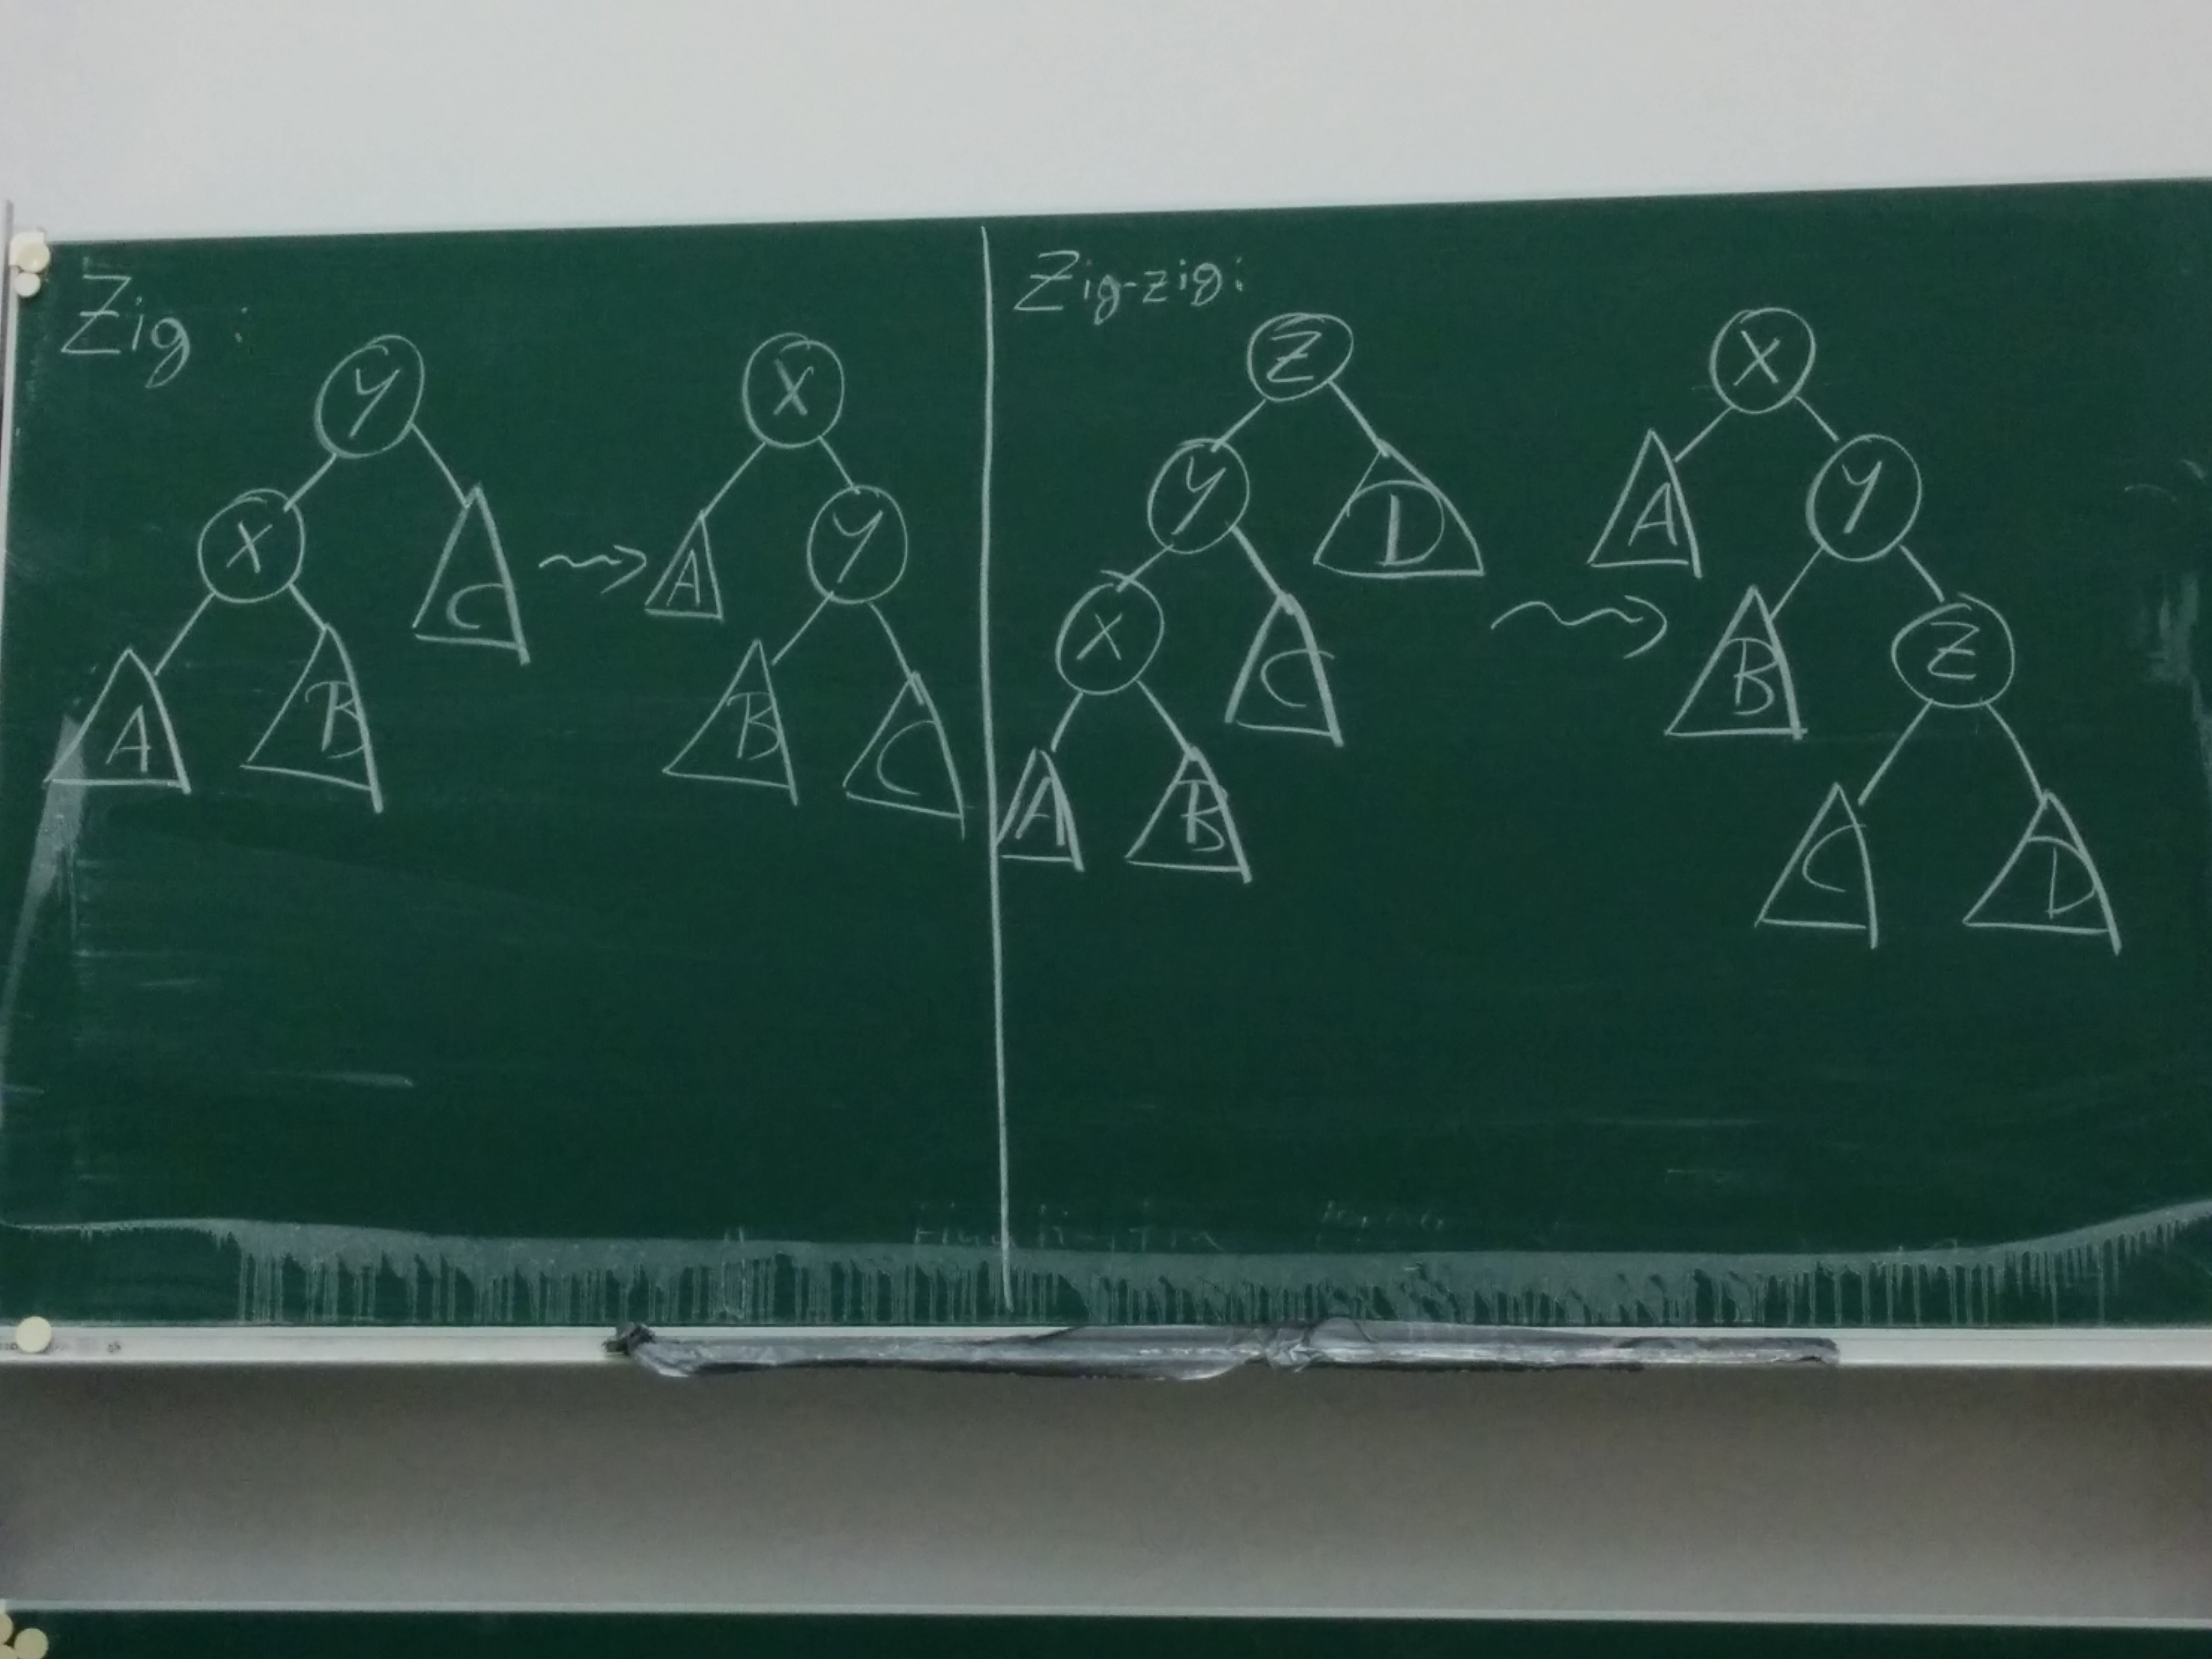
\includegraphics[width=430px]{tree1.jpg}

%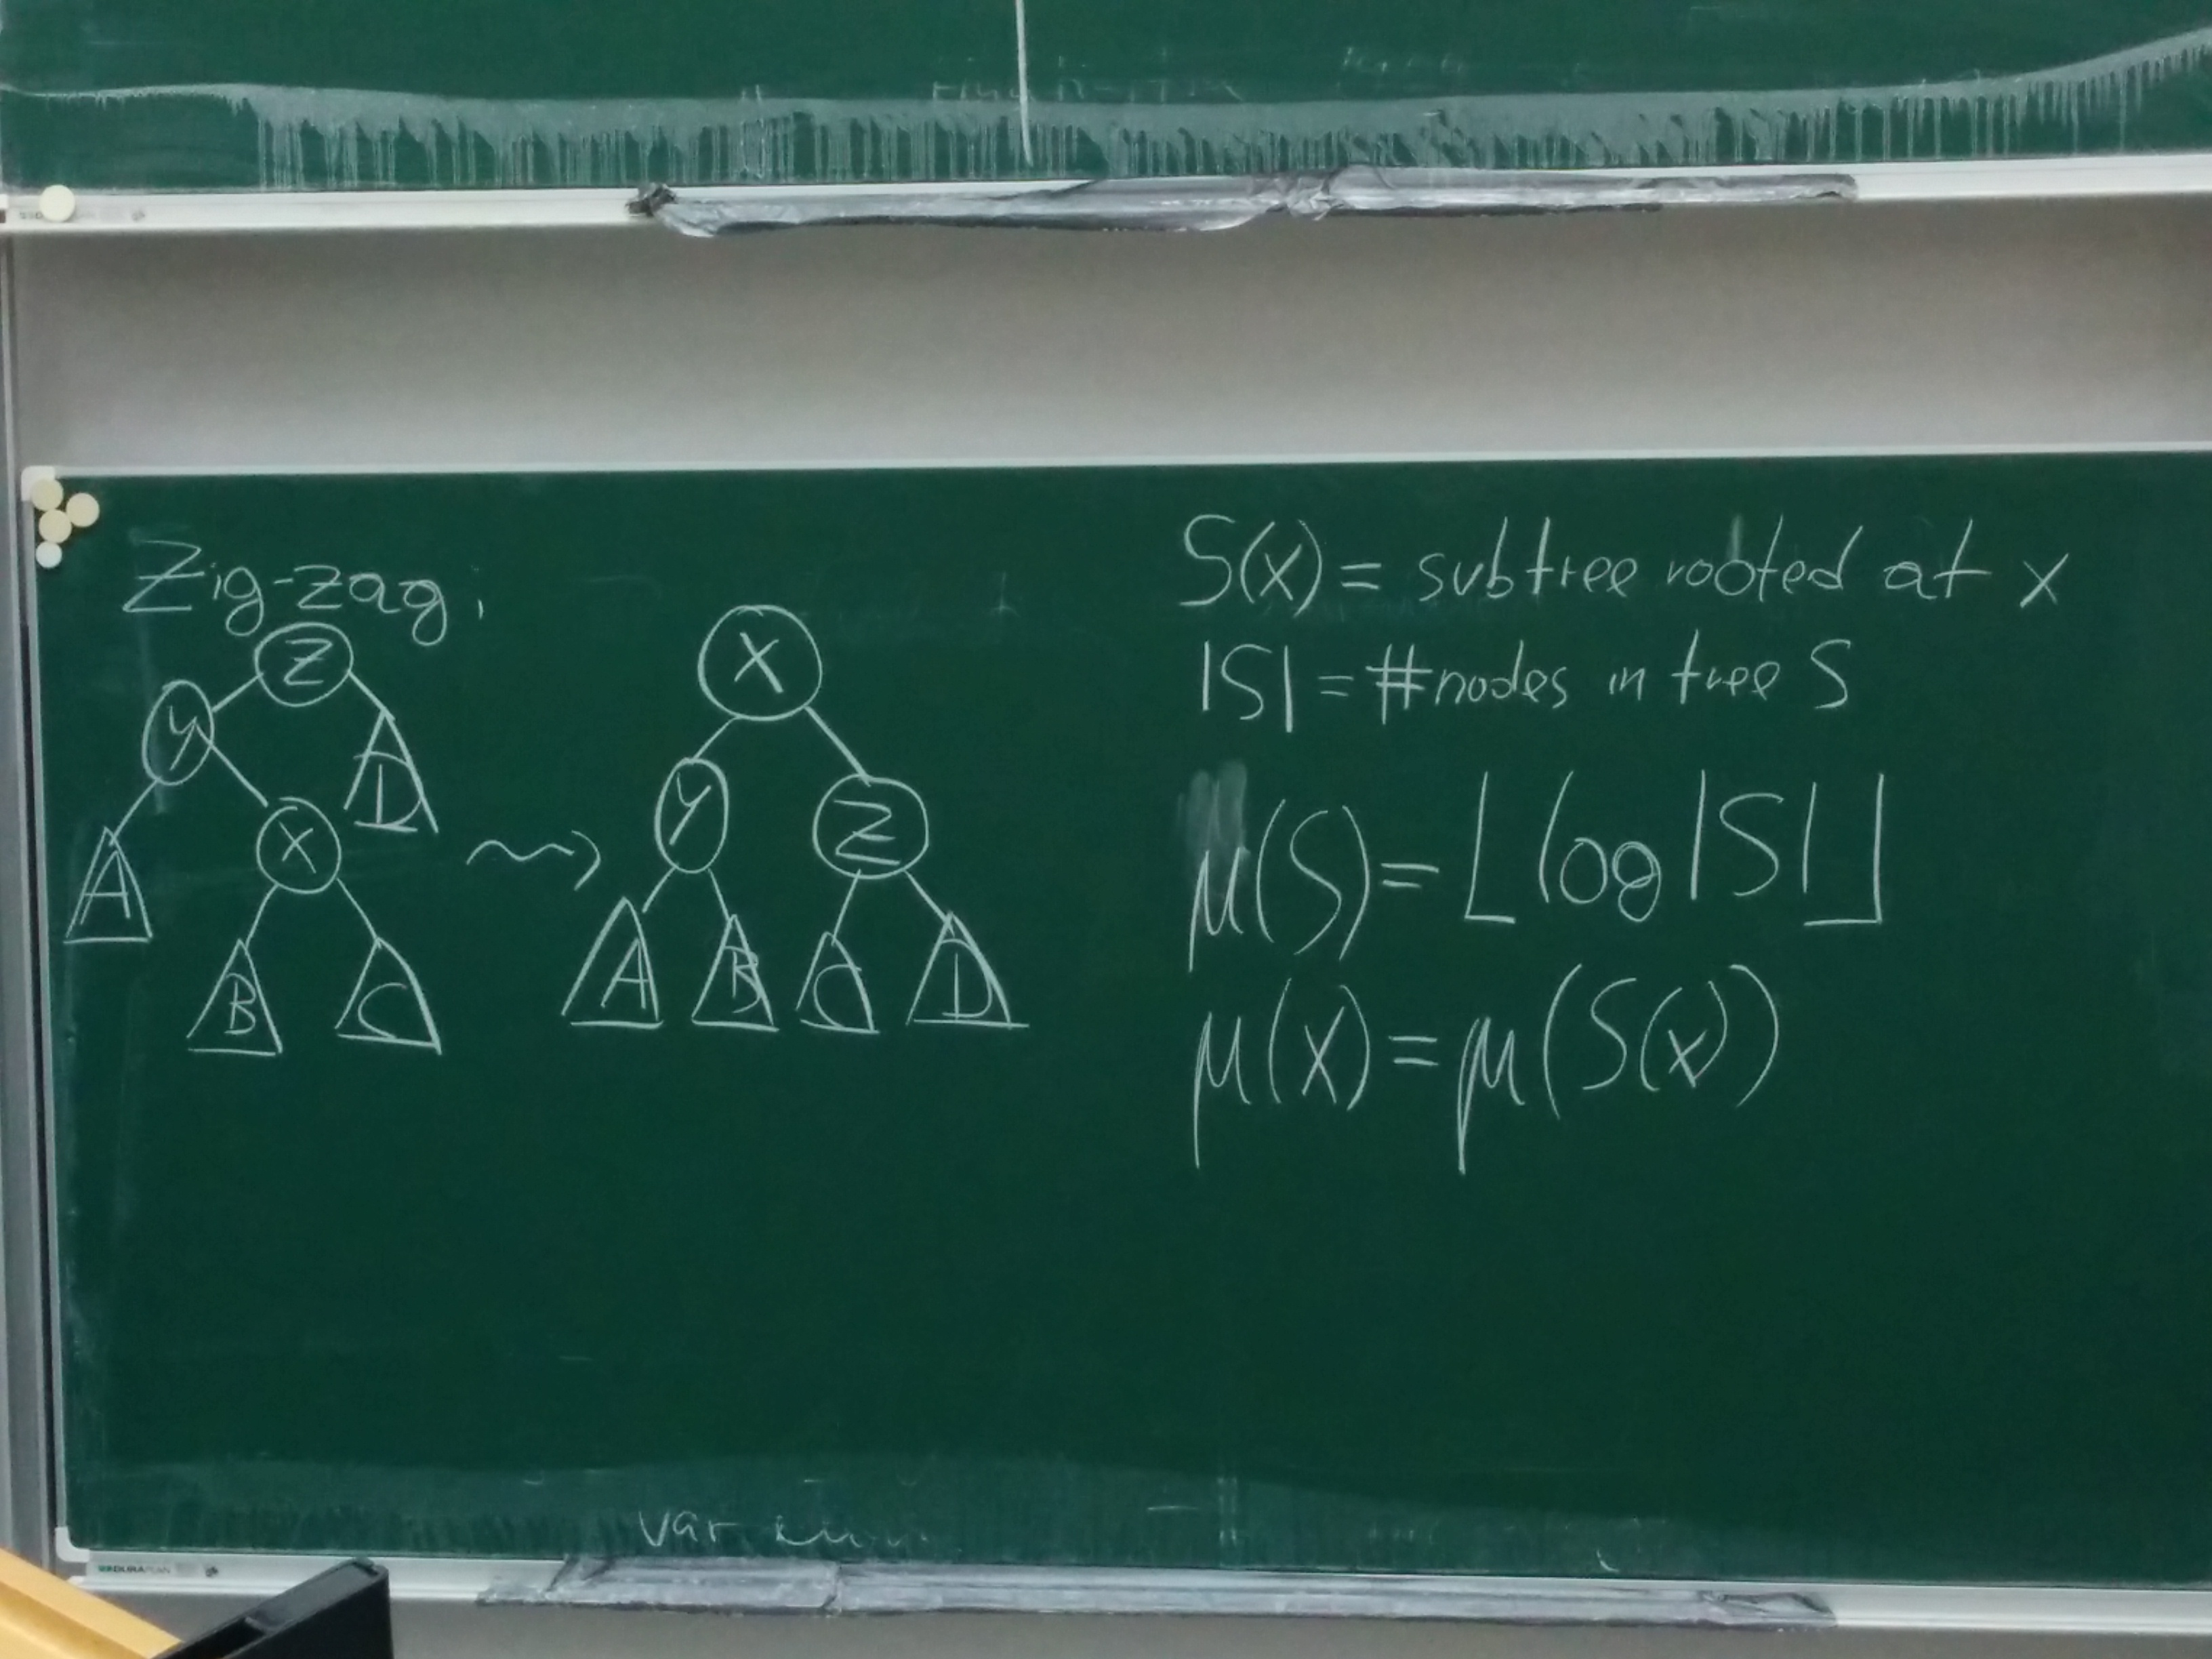
\includegraphics[width=430px]{tree2.jpg}

\begin{mylemma}
Let $x$ be the node that becomes root after a splay operation on tree $T$. We need to spent at most

$$3(\mu(T)-\mu(x)) + 1$$

tokens to pay for all steps and maintain the credit invariant.
\end{mylemma}
\begin{proof}
The cost of finding $x$ is proportional to the cost of rotating $x$ to the root, so we can concentrate on the latter.

For a fixed rotation, let $\mu$ and $\mu'$ denote the weight of a node before and after the rotation. We show:

\begin{enumerate}
\item In a zig-case, we need to pay at most $3(\mu'(x) - \mu(x)) + 1$ tokens.
\item In zig-zig or zig-zag case, we need to pay at most $3(\mu'(x)-\mu(X))$ tokens.
\end{enumerate}

$$[3(\mu'(x)-\mu(x))+3(\mu''(x)-\mu'(x)) + \ldots = 3(\mu(T)-\mu(x))+1] \text{ (telescoping sum)}$$

\paragraph{Proof of (i):} We have that $\mu(y) = \mu'(x)$, and $\mu'(y) \le \mu'(x)$. We have to pay:

\begin{align*}
\underbrace{(\mu'(x) - \mu(x))}_\text{credit inv. for $x$} \quad + \quad \underbrace{(\mu'(y)-\mu(y))}_\text{credit inv. for $y$} \quad + \quad \underbrace{1}_\text{for paying the rotation}  
& \le \mu'(x) -\mu(x) + 1 \\
& \le 3(\mu'(x) - \mu(x)) + 1
\end{align*}

\paragraph{Proof of (ii):} Consider a zig-zag. We need

$$C = \mu'(x) - \mu(x) + \mu'(y) - \mu(y) + \mu'(z) - \mu(z) + 1$$

tokens. Since $\mu'(x) - \mu(z)$, this simplifies to:

\begin{align*}
C & \le \mu'(y) - \mu(x) + \mu'(z) - \mu(y) + 1 \\
& \le \mu'(x) - \mu(x) + \mu'(x) - \mu(x) + 1 \\
& = 2(\mu'(x) - \mu(x)) + 1
\end{align*}

If $\mu(x) - \mu(x) > 0$, this is at most $3(\mu'(x) - \mu(x))$ and we are done. What if $\mu(x) = \mu(x)$? We show that $\mu(x)=\mu(x)$ implies that $C\le 0$, so we have to spend $0 \le 3(\mu'(x)-\mu(x)$.

By contradiction, assume $\mu'(x)=\mu(x)$ and $C\ge 1$. That means $\mu'(x)=\mu(x)$ and $(\mu'(x)+\mu'(y)+\mu'(z) \ge \mu(x)+\mu(y)+\mu(z)$.

Since $\mu(x)=\mu'(x)=\mu(z)$, we have that $\mu(y) = \mu(x) = \mu(z)$. So, the inequality simplifies to

$$\mu'(y) + \mu'(z) \ge 2\mu'(x),$$

which implies $\mu'(x) = \mu'(y) = \mu'(z) = \mu(x) = \mu(y) = \mu(z)$.

Consider $a = |S(x)|$ before rotating, and $b = |S(z)|$ after rotating.

Then $\underbrace{\lfloor \log a \rfloor}_{=\mu(x)} = \underbrace{\lfloor\log a + b + 1\rfloor}_{=\mu'(x)} = \underbrace{\lfloor \log b \rfloor}_{=\mu'(z)}$

For $a \le b$, $\mu'(x) = \lfloor \log a + b + a \rfloor \ge \lfloor \log 2a \rfloor \ge 1 + \lfloor \log a \rfloor > \lfloor \log a \rfloor$.

So $C \le 0$.
\end{proof}

\begin{mytheorem}
For an initially empty splay tree, a sequence of $m$ insertions/removals/searches with $n$ inserts costs $O(m \log n)$.
\end{mytheorem}
\begin{proof}
Every splay step pays $O(\log n)$ tokens to perform all operations. When inserting a node, we have to put $\log n$ tokens on its account for the credit invariant.
\end{proof}

\section{Heaps}

\begin{itemize}
\item Sorted sequences with restricted access patterns.
\item Elements have keys (priorities) as usual
\end{itemize}

A \emph{non-addressable priority queue} $Q$ supports:
\begin{itemize}
\item ${insert}(e, Q)$
\item ${min}(Q)$: return element with smallest key
\item ${delete\_min}(Q)$: remove smallest element
\item ${build}(e_1, \ldots, e_n)$: creates a priorirty queue with elements $e_1, \ldots, e_n$
\end{itemize}

A handle $h$ is a pointer to an element stored in $A$.
An \emph{addressable priorirty queue} $Q$ supports:
\begin{itemize}
\item ${insert}(e, Q)$: returns a handle to inserted element
\item ${remove}(h, Q)$: remove the element pointed by $h$
\item ${min}(Q)$
\item ${delete\_min}(Q)$
\item ${build}(e_1, \ldots, e_n)$
\item ${decrease\_key}(h, k, Q)$: replaces the key of $h$ with $k$ (must be smaller than old key)
\item ${union}(Q_1, Q_2)$: merges the priority queues $Q_1$ and $Q_2$
\end{itemize}

\subsection{Binary Heaps}

\begin{itemize}
\item It is a maximally balanced binary tree
\item Last level is left-aligned
\item One element per node
\item Heap-ordered: key at node $v$ is smaller than all keys in descendants of $v$
\item Can be stored as an array
\end{itemize}

\begin{lstlisting}[mathescape]
${insert}(e, Q)$:
    put $e$ at next free position in node $v$
    sift_up(v)
    
${sift\_up}(v)$:
    $w \gets {parent}(v)$
    if ${key}(v) > {key}(w)$, return
    else
        swap elements of $v$ and $w$
        ${sift\_up}(w)$
\end{lstlisting}

\begin{lstlisting}[mathescape]
${delete\_min}(Q)$:
    swap elements of root and last element in order
    delete last element
    ${sift\_down}({root})$

${sift\_down}(v)$:
    if $v$ is leaf, return
    $w \gets$ smallest child of $v$
    if ${key}(v) < {key}(w)$, return
    else
        swap contents of $v$ and $w$
        ${sift\_down}(w)$
\end{lstlisting}

\paragraph{Build: } Let $e_1, \ldots, e_n$ be the elements of the heap. Put the elements in any order and call ${heapify}({root})$.
\begin{lstlisting}[mathescape]
${heapify}(v)$:
    if $v$ has left child $w$:
        ${heapify}(w)$
    if $v$ has right child $w'$:
        ${heapify}(w')$
    ${sift\_down}(v)$
\end{lstlisting}

\paragraph{Cost: } A ${sift\_down}$ on level $i$ costs not more than $\log n -i$ steps. The total cost is given by:

\begin{align*}
\sum_{i = 0}^{\lfloor \log n \rfloor} 2^i (\log n - i) \\
& = \sum_{j = 0}^{\lfloor \log n \rfloor} 2^i (\log n - j) j \\
& = n \cdot \underbrace{\sum_{j = 0}^{\lfloor \log n \rfloor} \frac{1}{2^j} \cdot j}_{\le 2} \\
& = O(n)
\end{align*}

\begin{align*}
\sum_{j=0}^\infty \frac{j}{2^j} = \sum_{j \ge 1} \frac{j}{2^j} & = \sum_{j \ge 1} \frac{1}{2^j} + \sum_{j \ge 2} \frac{1}{2^j} + \sum_{j \ge 3} \frac{1}{2^j} + \ldots  \\
& = \sum_{j \ge 1} \frac{1}{2^j} + \frac{1}{2} \sum_{j \ge 2} \frac{1}{2^{j-1}} + \frac{1}{4} \sum_{j \ge 3} \frac{1}{2^{j-2}} + \ldots \\
& = \sum_{j \ge 1} \frac{1}{2^j} + \frac{1}{2} \sum_{j \ge 1} \frac{1}{2^j} + \frac{1}{4} \sum_{j \ge 1} \frac{1}{2^j} + \ldots \\
& = \underbrace{\sum_{j \ge 1} \frac{1}{2^j}}_{=1} \left ( 1 + \frac{1}{2} + \frac{1}{4} + \ldots \right ) \\
& \le 2
\end{align*}






%\newpage \section{Fibonacci Heaps}

\paragraph{Representation:}

\begin{itemize}
\item Forest of (arbitrary) heap-ordered trees
\item Min-pointer to smallest element ($\implies {min}(Q) = O(1)$)
\item Roots are connected by a linked list, called the \emph{root list}
\end{itemize}

\paragraph{Every node contains:}

\begin{itemize}
\item One element
\item Its rank (= \# children)
\item Pointers to parent, left and right sibling, and to one child
\item A flag (marked or not) used in ${decrease\_key}$.
\end{itemize}

\paragraph{Operations:}

\begin{itemize}
\item ${insert}(e,Q)$: Add new tree with one node $e$ to root list and update the ${min}$ pointer $\implies O(1)$.
\item ${union}(Q_1, Q_2):$ Splice the root lists and update the ${min}$ pointer $\implies O(1)$.
\item ${remove}(h, Q):$ ${decrease\_key}(h, -\infty, Q)$, then, ${delete\_min}(Q)$. 
\end{itemize}

\begin{lstlisting}[mathescape]
${delete\_min(Q)}$
    Delete min-node and add all its children to the root list
    Create and unbounded array $A$ storing handles to roots
    Traverse the root list. Let $v$ be a root and $r$ its rank:
        while($A[r] \neq \bot$):
            Let $w = A[v]$, so ${rank}(v)=r={rank}(w)$.
            Combine $v$ and $w$ into a new tree by making either $v$ a child
            of $w$ or vice versa.
            $A[v] \gets \bot$
            $r \gets r + 1$
        $A[v] \gets V$
    Traverse $A$ once more and find ${min-node}$ to update the pointer
            
\end{lstlisting}

${Decrease\_key}$ can be defined as follows:

\begin{lstlisting}[mathescape]
${decrease\_key(h, k, Q)}$
    Cut subtree at $h$ and make it a new root
    Update its key and update the ${min\_pointer}$. $\implies O(1)?$
\end{lstlisting}

However, this allows too ``wild'' shapes for the trees.



\begin{lstlisting}[mathescape]
Repair (Cascading Cuts):
    When node $v$ is cut, let $w$ be its parent.
    while($w$ is marked):
        Unmark and cut $w$
        $w \gets$ (old) parent of $w$
\end{lstlisting}

\subsection{Amortized Analysis}

\paragraph{Credit Invariant:} Each root holds one token and each marked node holds two tokens.

Let $R$ be the maximal rank of a node in the Fibonacci Heap.

\begin{mylemma}
${decrease\_key}$ needs to pay $O(1)$ credits to perform all its operations and maintain the credit invariant.
\end{mylemma}
\begin{proof}
The methods marks (at most) one element and we can spend the two tokens for this marking. The first cut costs $O(1)$. Any further cut turns a marked node into a root, so one token becomes free and we spend it to pay for the cut.
\end{proof}

\begin{mylemma}
${delete\_min}$ needs to pay $O(R)$ credits to pay for all its operations and to maintain the credit invariant.
\end{mylemma}
\begin{proof}
We need to pay $O(R)$ credits to make the children of min-node roots and give them one token each. The array $A$ has size $O(R)$, and ${delete\_min}$ can pay for initialization.

The running time of the loop is $O(R + \# {combines})$. Each combine turns some root into a non-root, so we can use its token to pay or the combine. Finding the min-pointer costs at most $O(R)$ additional operations.
\end{proof}

It remains to show that $R = O(\log n)$.

\paragraph{Fibonacci Numbers:}
\begin{itemize}
\item $F_0 = 0, F_1 = 1, \forall i \ge 2, FI = F_{i-1} + F_{i - 1}$
\item 0,1, 1,2,3,5,8,13,21, \ldots
\end{itemize}

\begin{mylemma}
$F_{i + 2} \ge \left ( \frac{1 + \sqrt{5}}{2} \right )^i \ge 1.618^i$ (homework).
\end{mylemma}

\begin{mylemma}
Let $v$ be a node of rank $i$. Then, the subtree rooted at $v$ has at least $F_{i+2}$ nodes. In particular, if the FH has $n$ nodes, each rank is bounded by $1.4404 \log n$.
\end{mylemma}
\begin{proof}
Let $v$ be a node of rank $i$. Let $w_1, \ldots, w_i$ be its children, sorted in order when they became children of $v$. For $w_j, 1 \le j \le i$, $w_j$ became child of $v$ through a combine in ${delete\_min}$. So, the rank of $w_j$ at that time was at least $j - 1$, because $w_1, \ldots, w_{j-1}$ were children of $v$ and combine only merges roots of same rank. Because $w_j$ has lost at most one child since then, ${rank}(w_j) \ge j-2$.

Let $S_i$ be the minimum number of nodes in a subtree with a root of rank $i$. We have $S_0 = 1, S_i \ge 2$ and $\forall i \ge 2, S_i \ge 2 + S_0 + S_1 + \ldots + S_{i-2}$.

We have that $S_i \ge F_{i+2}$ (homework).

For the second claim, for any ode of tank $i$, we have $F_{n+2} \le n \iff 1.618^n \le n \iff i \le 1.4404 \log n$.
\end{proof}

\section{Union-find}

We want to represent a collection of \emph{disjoint} sets $S_1, \ldots, S_k$. Each set $S_i$ has a representative $r_i \in S_i$. Our data structure suports:

\begin{itemize}
\item ${make\_set}(x):$ Create a new set $\{x\}$
\item ${union}(x, y):$ Combine $S_i$ and $S_j$, where $x \in S_i$ and $y \in S_j$, into a new set $S_i \cup S_j$ and pick some element of the union as representative.
\item ${find}(x):$ return the representative of the set containing $x$
\end{itemize}
 
\paragraph{Application:} Find the connected components of a graph $\implies$ minimum spanning tree.

\paragraph{Representation: }
\begin{itemize}
\item Forest of (arbitrary) trees, one per set
\item One element per node. Root contains the representative.
\item Only pointer to the parent. Root points to itself.
\end{itemize}

Naive implementation of ${make\_set}$, ${union}$, ${find}$ is clear. Efficiency? Bad, because trees can degenerate.

\paragraph{Optimization 1: } ``Union by ranks''. Merge the less deep tree into the deeper tree.


%\section{Graph Algorithms}

\subsection{Connectivity}

We have a directed graph $G=(V,E)$, \emph{simple} (no loops or multi edges).

$$n = |V|, m = |E|$$

\paragraph{(Directed) Path of length $k$}

\paragraph{(Directed) Cycle of length $k+1$: } Directed path of length $k$ + find edge $(v_{k+1}, v_1)$.

\paragraph{Simple path, simple cycle: } No vertex appears twice on the path/cycle.

\begin{itemize}
\item Graph $G=(V, E)$ is \emph{strongly connected} if it has a $(v,u)$-path and $(u,v)$ path for all $v,w \in V$.

\item Undirected graph $G$ is $k$-connected ($k$-vertex connected) if removal of at most $k-1$ vertices (and all incident edges) keeps the graph connected. $k$-edge connected similar, but for edge removal.

\item An inclusion-maximal strongly connected subgraph is a strongly connected component. Same for $k$-connected and $k$-edge-connected. \emph{Intuitively, it cannot be extended with more vertices/edges and maintain the same property.}
\end{itemize}

\subsection{DFS Framework}

\begin{lstlisting}[mathescape]
Input: Graph directed or indirected, $G=(V,E)$
Data Structure:
    Stack S (for vertices on the DFS path)
    Vertex array "incoming" (for first incoming edge)
    Vertex & edge markings

for each $s \in V$ do:
    mark S, set incoming[s] $\gets$ nil, push $s \rightarrow S$
    root(S)
    
    while S is not empty do:
        $v \gets top(S)$
        if $\exists$ unmarked $e = (v,w) \in E$ then
            mark $e$
            if $w$ is unmarked:
                mark $w$, set incoming[$w$] $\gets$ e, push $w$
                traverse(v,e,w)
        else:
            $w \gets pop(S)$
            backtrack(w, incoming[w], top(S))
\end{lstlisting}

Sequence in which vertices are discovered/marked: $v_1, v_2, \ldots, v_n$.
\begin{itemize}
\item \emph{DFS-number} of $v_i$ as $DFS(v_i) = i$.
\item \emph{DFS-number} of $(v,w$) is $DFS((v,w)) = DFS(v)$.
\item \emph{DFS-order} $\preceq$ on $V$ or $E$ by:
\end{itemize}

$$DFS(p) \le DFS(q) \iff p \preceq q$$

$$DFS(p) < DFS(q) \iff p \prec q$$

\paragraph{Edge Classes: } If $(v,w)$ is marked, it becomes a
\begin{itemize}
\item \emph{tree edge} if $w$ is unmarked
\item \emph{back edge} if $w$ is marked, $w \preceq v, w \in S$
\item \emph{cross edge} if $w$ is marked, .......
\end{itemize}

\subsection{Undirected DFS}

\begin{itemize}
\item Edges are traversed independently of direction.
\item Replace the check of $\exists$ unmarked $e=(v,w) \in E$ with: $e=(v,w) \in E$ or $e=(w,v) \in E$.
\item In undirected DFS, there are no cross and no forward edges (homework!).
\end{itemize}

\subsection{Connected Components}

\begin{lstlisting}[mathescape]
root(s):
    $c \gets s$. component[S] $\gets c$

traverse(v,e,w):
    component[e] $\gets c$, component[w] $\gets c$.
\end{lstlisting}

\begin{itemize}
\item Component is represented by first discovered vertex.
\item Output: Array ``component'', pointing to representing vertex of the component
\item Requires $O(n+m)$ time, $O(n+m)$ space.
\end{itemize}

\subsection{2-connected Components}

\begin{mylemma}
For an undirected graph $h$, edges $e, e' \in E$ are in a 2-connected component if, and only if, there is a simple undirected cycle that contains both $e$ and $e'$. The set of 2-connected components is a partition of the $E$.
\end{mylemma}
\begin{proof}
If a cycle exists, then $e$ and $e'$ are in a 2-connected component.

Subdivide $e$ and $e'$ each with a new vertex. Component is still 2-connected.
Existence of a simple cycle follows from Menger's Theorem.
\end{proof}

\begin{mytheorem}[Menger's Theorem]
In a 2-connected undirected graph with at least 2 edges there are two vertex-disjoint paths between every pair of vertices.
\end{mytheorem}

\begin{proof}[Proof for partition statement]
For the partition statement, assume by contradiction $e$ is in two 2-connected components. There is a simple undirected cycle between $e'$ in one component and $e''$ in the other component. 
There are simple cycles, and they exist for every pair in the union of components. But components must be inclusion-maximal. Contradiction.
\end{proof}

\subsection{Undirected DFS for 2-connected components}

\begin{itemize}
\item Stack $S_E$ for edges in unfinished (or open) components
\item Stack $C$ for open components (represented by first edge)
\item Output: Array ``component'' pointing to representing edge
\end{itemize}

\begin{lstlisting}[mathescape]
traverse(v,e,w):
    push $e \rightarrow S_E$
    if $e$ is free edge then push $e \rightarrow C$
    if $e$ is back edge then:
        while $w \prec$ top(c) do:
            pop(c)

backtrack(w,e,v):
    if $e = top(c)$ and $e \neq nil$ then:
        pop(c)
        repeat
            $e' \gets pop(S_E)$
            component[$e'$] $\gets e$
        until $e = e'$.
\end{lstlisting}


%\section{Matroids}

Recall minimum spanning trees, that can be solved using a greedy algorithm. Matroids are a broad generalization construction. It captures the notion of linear dependence.

\begin{mydefinition}
A matroid is a pair $(S, I)$, where $S$ is a finite set and $I$ is a family of subsets of $S$, such that:
\begin{enumerate}
\item if $J \in \mathcal{I}$ and $I \subseteq J$, then $I \in \mathcal{I}$.
\item if $I, J \in \mathcal{I}$ and $|I| < |J|$, then there is an $x \in J-I$ with $I \cup \{x\} \in \mathcal{I}$.
\end{enumerate}

$I \in \mathcal{I}$ is called \emph{independent set}, and $I' \subseteq S$ with $I' \notin \mathcal{I}$ is a \emph{dependent set}.
\end{mydefinition}

\paragraph{Examples}
\begin{enumerate}
\item $V$ is a vector space, finite $S \subseteq V$, $\mathcal{I} \subseteq 2^S$ family of linearly independent subsets of $S$. That's why $I \in \mathcal{I}$ is called an independent set.
\item $S$ are rows of a matrix $A$, $\mathcal{I} \subseteq 2^S$ family of linear independent subsets of $S$.
\item $G = (V, E)$ undirected connected graph, $S = E$, $\mathcal{I}$ is the set of forests of $G$. Also called \emph{graphical matroid}.
\item $G = (V, E)$ undirected connected graph, $S = E$, $\mathcal{I} \subseteq 2^E$ such that $E' \in \mathcal{I}$ with $G' = (V, E-E')$ stays connected.
\item $S$ set of elements, $\mathcal{I} \subseteq 2^S$ containing all sets $J \subseteq S$ with $|J| \le k$ for some given $k > 0$. Also called \emph{uniform matroid}.
\end{enumerate}

\begin{mydefinition}
A \emph{weighted matroid} has a given cost function $c: S \rightarrow \mathbb{R}$.
\end{mydefinition}

\begin{mydefinition}
A \emph{maximal independent set} $J \in I$ is such that $\forall x \in S-J, J \cup \{x\} \notin \mathcal{I}$, and is called \emph{basis}.
\end{mydefinition}

Matroid are exactly the structures in which a greedy algorithm fins a basis of minimum cost.

\begin{lstlisting}[mathescape]
Greedy algorithm matroid:
    $J \gets \emptyset$
    while $\exists x \in S$ such that $J \cup \{x\} \in I$ do
        let $X = \{x \in S | J \cup \{x\} \in \mathcal{I}\}$ and pick $x^* = \arg\min_{x \in X} c(x)$.
        $J \gets J \cup \{x*\}$ 
\end{lstlisting}

\begin{mytheorem}
A set system $(S, \mathcal{I})$ satisfying axiom (i) of matroids is a matroid (i.e. satisfies (ii)) if and only if for all cost functions the greedy algorithm finds a basis
of minimum cost.
\end{mytheorem}

We show that a greed algorithm works in a more general sense.

\begin{mydefinition}
A \emph{cycle} of a matroid $(S, \mathcal{I})$ is an inclusion-minimal dependent set.
\end{mydefinition}

\begin{mydefinition}
A \emph{cut} of a matroid $(S, \mathcal{I})$ is an inclusion-minimal subset of $S$ intersecting all bases.
\end{mydefinition}

For graphic metroids, \emph{cycles} in the metroid are exactly simple cycles of $G$. A cut in the metroid is a subset of the cuts in the graph, because it has to be inclusion-minimal (captures only the ``essential'' cuts).

\subsection{Greedy and Dual Greedy algorithms}

\paragraph{Blue rule:} Find a cut with no blue element. Then, pick an element of this cut of minimum cost and color it blue.

\paragraph{Red rule:} Find a cycle with no red element. Then, pick an element of the cycle of maximum cost and color it red.

\begin{mytheorem}
If we start with an uncolored weighted matroid, and apply the blue and red rules (in any order) until neither applies, then the blue elements are a basis of minimum cost.
\end{mytheorem}

For the proof we use duality.

\begin{mydefinition}
For a matroid $(S, \mathcal{I})$, the \emph{dual matroid} is $(S, \mathcal{I}^*)$ with $\mathcal{I}^* = \{ J \subseteq S | J \cap B = \emptyset \text{ for some basis $B$ of $\mathcal{I}$} \}$. $J^*$ is basis in $\mathcal{I}^*$ iff $S-J^*$ is basis in $\mathcal{I}$. Note: $\mathcal{I}^{**} = \mathcal{I}$.
\end{mydefinition}

For example, (3) and (4) above are dual (graphic metroid and sets of edges that upon removal keep $G$ connected).

\paragraph{Note:}
\begin{itemize}
\item Usually $J \in \mathcal{I}$ does not imply $J \in \mathcal{I}^*$. Empty set is in both matroids. 
\item Cuts in $(S, \mathcal{I})$ are cycles in $(S, \mathcal{I}^*)$.
\item Blue rule in $(S, \mathcal{I})$ is red rule in $(S, \mathcal{I}^*)$ with reversal ordering of costs.
\end{itemize}

\begin{mydefinition}
An \emph{acceptable coloring} $(B, R)$ with $B \in \mathcal{I}$, $R \in \mathcal{I}^*$ is \emph{total} if $B \cup R = S$, i.e., both $R$ and $B$ are bases in the matroid and its dual. It \emph{extends} acceptable coloring $(B', R')$ if $B' \subseteq B, R' \subseteq R$.
\end{mydefinition}

\begin{mylemma}
Every acceptable coloring has a total extension.
\end{mylemma}
\begin{proof}
Let $U^*$ be a basis of $\mathcal{I}^*$ and $R\subseteq U^*$. Then, let $U = S - U^*$, so $U$ is a basis of $\mathcal{I}$. Since $|B| < |U|$, select $x \in U-B$ and add it to $B$ such that $B \cup \{x\} \in \mathcal{I}$. This is possible by axiom (ii) of matroids. Since all bases have same cardinality, again by axiom (ii), the resulting set $\hat{B}$ is a basis disjoint from $R$. Then, total extension is given by $(\hat{B}, S - \hat{B})$.
\end{proof}

\begin{mylemma}
A cut and a cycle cannot intersect in one element.
\end{mylemma}
\begin{proof}
Suppose they do intersect in element $X$. Color cycle without $x$ blue, and color the cut without $x$ red. This is an acceptable coloring, that can be extended to total, by previous lemma. Then, it is impossible to color $x$. So either cycle is blue (not in $\mathcal{I}$), or cut is red (not in $\mathcal{I}^*$). Contradiction.
\end{proof}

\begin{mydefinition}
Suppose $B \in \mathcal{I}$, $ B \cup \{x\} \notin \mathcal{I}$. Then, $B \cup \{x\}$ contains a minimal dependent subset $C$, the \emph{fundamental cycle} of $x$ and $B$. Note: $x \in C$.
\end{mydefinition}

\begin{mylemma}
For a total acceptable coloring $(B,R)$,
\begin{enumerate}
\item let $x \in R$ and $y$ in a fundamental cycle of $x$ and $B$. If we exchange colors of $x$ and $y$, the resulting coloring is acceptable.
\item let $y \in B$ and $x$ in a fundamental cut of $y$ and $R$. If we exchange colors of $x$ and $y$, the resulting coloring is acceptable.
\end{enumerate}
\end{mylemma}
\begin{proof}
By duality, we show only (i). If $y = x$, then the coloring will be the same. Otherwise, $C - \{y\} \in \mathcal{I}$, because $C$ is inclusion-minimal. We extend $C - \{y\}$ by adding elements of $B$ until we get a basis $B'$. Then $B' = (B - \{y\}) \cup \{x\}$, and the total acceptable coloring $(B', S-B')$ results from exchanging colors of $x$ and $y$.
\end{proof}

\begin{mydefinition}
A total acceptable coloring is \emph{optimal} if $B$ is a minimum-cost basis, or equivalently, $R$ is a maximal-cost basis in the dual matroid.
\end{mydefinition}

\begin{mylemma}
If $(B,R)$ has an optimal total extension, then this is maintained after the execution of the blue or red rule.
\end{mylemma}
\begin{proof}
By duality, we show for the blue rule. Let the optimal total extension be $(\hat{B}, \hat{R})$. $A$ is cut without blue elements, $x \in A$ is the minimum-cost element. If $x \in \hat{B}$, then done, so let $x \in \hat{R}$. $C$ is the fundamental cycle of $x$ and $\hat{B}$. Then, $|A \cap C| \ge 2$, so there is $y \in A \cap C, y \neq x$. Also, $y \notin B, y \in \hat{B}$. By exchange lemma, we switch colors of $x$ and $y$ in $(\hat{B}, \hat{R})$, and this new total acceptable coloring $(\hat{B}', \hat{R}')$ extends $(B \cup \{x\}, R)$. $\hat{B}'$ has minimum cost since $c(y) \ge c(x)$, by blue rule.
\end{proof}

\begin{mylemma}
If an acceptable coloring $(B, R)$ is not total, then either the blue or red rule can be applied.
\end{mylemma}
\begin{proof}
Let $x$ be an uncolored element. $(B,R)$ has total extension $(\hat{B}, \hat{R})$. By duality, assume $x \in \hat{B}$. Then $C$ is a fundamental cut of $x$ and $\hat{R}$. Since every $y \in C$ with $y \neq x$ are in $\hat{R}$, then $y \notin B$. Here the blue rule applies to $C$.
\end{proof}


%\begin{proof}[\textbf{Proof of Theorem 2:} ]
%\end{proof}


%\section{Network Flows}

We consider directed capacitated network $G = (V, E, c, s, t)$.
\begin{itemize}
\item $V$ vertices, $E$ edges, $s,t \in V$, $s$ \emph{source}, $t$ \emph{sink}
\item $c: E \rightarrow \mathbb{R}_{\ge 0}$ denote \emph{edge capacities}
\end{itemize}

\begin{mydefinition}
A \emph{flow} F is a function $f: E \rightarrow \mathbb{R}$ that satisfies
\begin{enumerate}
\item Capacity Constraint: $\forall e \in E: 0 \le f(e) \le c(e)$ 
\item Conservation of Flow: $\forall v \in V - \{s,t\}: \sum_{(x,v) \in E} f((x,v)) = \sum_{(v,y) \in E} f((v,y))$
\end{enumerate}

\end{mydefinition}

\begin{mydefinition}[A different view]
A \emph{flow} is a function $f: V \times V \rightarrow \mathbb{R}$ with
\begin{enumerate}
\item $\forall (u,v) \in E: f(u,v) \le c(u,v)$, and, $\forall (u,v) \notin E: f(u,v) \le 0$
\item $f(u, v) = - f(v,u)$
\item $\forall u \in V - \{s,t\}: \sum_{v \in V} f(u,v) = 0$
\end{enumerate}
\end{mydefinition}

\begin{mydefinition}[Extension to vertex sets]
Let $U, W \subseteq V$, then $f(U,W) = \sum_{u \in U} \sum_{w \in W} f(u,w)$.
\end{mydefinition}

\begin{mydefinition}
The \emph{value} of a flow $|f| = f(\{s\}, V) = f(V, \{t\})$.
\end{mydefinition}

\begin{mydefinition}
An $s$-$t$-cut in graph $G$ is a partition of the vertex set $V$ into sets $S, T$ such that $S \cap T \neq \emptyset$, $S \cup T = V$, and $s \in S$, $t \in T$.
\end{mydefinition}

\begin{mylemma}
If $(S,T)$ is an $s$-$t$-cut in $G$, then $f(S,T) = |f|$.
\end{mylemma}
\begin{proof}
We first show that for $s$-$t$-cuts $(X \cup \{x\}, Y)$ and $(X, \{x\} \cup Y)$.
We are going to show that:

\begin{align*}
f(X \cup \{x\}, Y) &= f(X, \{x\}\cup Y) \\
f(X,Y) + f(x,Y) &= f(X,x) + f(X,Y) \\
f(x,Y) &= f(X,X) \\
f(x,Y) + f(x,X) &= 0 \\
f(x, X \cup Y) &= 0 && \text{[Conservation of flow]}
\end{align*}

Hence, all $s$-$t$-cuts have $f(S,T) = f(\{s\},V) = |f|$.
\end{proof}

\begin{mycorollary}
For any $s$-$t$-cut, we have that the value of the flow is upper bounded by the capacity of the cut:

$$|f| = f(S,T) = \sum_{u \in S} \sum_{v \in T} f(u,v) \le \sum_{u \in S} \sum_{v \in T} c((u,v)) = c(S,T)$$
\end{mycorollary}

\begin{mytheorem}[Max-Flow-Min-Cut [Ford \& Fulkerson]]
There is a flow $f$ such that $|f| = \min \{c(S,T) | (S,T) \text{is a $s$-$t$-cut}\}$.
\end{mytheorem}

\begin{mydefinition}[Residual Graph]
For a flow $f$ in network $G$, the residual graph $G_f$ has \emph{residual capacity}

\begin{align*}
\forall (u,v) \in V \times V, \\
& c_f(u,v) = \underbrace{c(u,v)}_{\text{$0$ for $(u,v) \notin E$}} - \; f(u,v)
\end{align*}
\end{mydefinition}

$G_f$ contains all edges $(u,v)$ with $c_f(u,v) > 0$. Intuitively, it  ``contains opposite edges''.

\paragraph{Observation:} Suppose we have a flow $f$ for $G$, and that we have a flow $f'$ for $G_f$, then $f + f'$ is a flow for $G$, such that $|f + f'| = |f| + |f'|$.

With the residual network, we can increase some flow and easily verify correctness.

\begin{enumerate}
\item Find a path from $s$ to $t$ in the residual graph
\item Identify smallest residual capacity on that path
\item Send this much flow.
\end{enumerate}

\begin{mydefinition}
An $s$-$t$-path $p = <e_1, \ldots, e_k>$ is called \emph{augmenting path}. The flow change on $p$ is $|f_p| = u = \min\{c_p(e_i) | 1 \le i \le k\}$. 

Then, $f_p(v_i, v_{i+1}) = u, f_p(v_{i+1}, v_i) = -u$ with $e_i = (v_i, v_{i+1})$, $v_1 = s$, $v_{k+1} = t$. And $f_p(u,v) = 0$ otherwise.
\end{mydefinition}

\subsection{Ford-Fulkerson Algorithm}

\begin{lstlisting}[mathescape]
    Initially $f \gets 0$
    while $\exists$ $s$-$t$-path in $G_f$ do
        Augment along $p: f \gets f + f_p$.
\end{lstlisting}

\begin{enumerate}
\item \textbf{Does this terminate?}
    In general, no, but for integer-valued capacities, yes. Every cut provides an upper bound on $|f|$, and we increase in unit amounts.
 
\item \textbf{Number of iterations?}
    At most $|f_{\max}|$
\end{enumerate}

\begin{mytheorem}[Max-Flow Min-Cut Theorem]
The following statements are equivalent:
\begin{enumerate}
\item $f$ is a maximum flow.
\item $f$ does not admit an augmenting path in $G_f$.
\item There exists an $s$-$t$-cut $(S,T)$ with $f(S,T) = c(S,T)$. 
\end{enumerate}
\end{mytheorem}
\begin{proof}
First, $(3) \implies (1)$. Since $\forall$ $s$-$t$-cut $(S,T)$, $|f| \le c(S,T)$.
Second, $(1) \implies (2)$. By Ford-Fulkerson algorithm.
Third, $(2) \implies (3)$. This means that in $G_f$, $s$ is not connected to $t$. For every $s$-$t$-path in $G$, consider the first edge $e=(u,v)$ with $c_f(u,v) = 0 = c(u,v) - f(u,v)$. Here $c(u,v) = f(u,v)$. Define $S = \{ v \in V | \exists \text{ $s$-$v$-path in $G_f$}\}$. Let $T = V - S$, then $(S,T)$ is an $s$-$t$-cut and $|f| = f(S,T) = c(S,T)$.  
\end{proof}

\subsection{Edmonds-Karp Algorithm}

Run the Ford-Fulkerson Algorithm and pick a path in $G_f$ with smallest number of edges.

\begin{mylemma}
In the Edmonds-Karp Algorithm, the shortest path distance $\mu_f(s,v)$ for all $v \in V$ in the residual network increases monotonically with every flow augmentation.
\end{mylemma}
\begin{proof}
Increase by $f_p$ yields $f(u,v) = c(u,v)$. Edges disappears, reverse edge appears.
Since $p$ is a shortest path, it rows top down. By pushing flow, we loose top-down edges in the process. This implies no vertex can decrease its level. After at most $m$ augmentations, distance $\mu_f (s,t)$ increases by at least 1. $\mu_f(s,t)$ can only increase to at most $n-1$. Therefore, the number of iterations is bounded by $n \cdot m$.

Each BFS-call to find augmenting paths takes time $O(m)$.
\end{proof}

\begin{mylemma}
The Edmonds-Karp Algorithm computes a maximum flow in time $O(n\cdot m^2)$.
\end{mylemma}


%\section{Preflow-push Algorithm}

\paragraph{Recall:} $G=(V,E,c,s,t)$ is a directed capacitated network. We have a flow $f$:

\begin{enumerate}
\item $\forall u,v \in V: f(u,v) = - f(u,v)$
\item $\forall u,v \in V: f(u,v) \le c(u,v)$
\item $\forall u\in V - \{s,t\}: \sum_{x \in V} f(x,u) = 0$
\end{enumerate}

Now we consider a different approach based on preflow. A \emph{preflow} $f: V \times V \rightarrow \mathbb{R}$ satisfies:
\begin{enumerate}
\item $f(u,v) = - f(v,u)$
\item $f(u,v) \le c(u,v) \gets$ capacity for $(u,v) \in E$, or $0$ for $(u,v) \notin E$.
\item $\forall u \in V - \{s\}, \sum_{x \in V} f(x,u) \ge 0$
\end{enumerate}

Condition (3) means that interior vertices can drop flow but cannot generate it. Incoming flow $\ge$ outgoing flow.

Let $\Delta_f(v) = \sum_{x \in V} f(x,v)$ be the \emph{excess} of preflow $f$ at $v \in V$.

\paragraph{Note:} Preflow is flow if $\forall v \in V - \{s,t\}, \Delta_f(v) = 0$ and $|f| = \Delta_f(t) = -\Delta_f(s)$.

\bigskip 

We define the residual graph $G_f$ for preflow $f$ exactly as before ($c_f(u,v) = c(u,v) - f(u,v)$).

\subsection{Labelings}

Labelings give a notion of height, where nodes are pushed up, forcing the flow into other nodes.

Preflow-Push Algorithm pushes more flow than possible. Eventually flow finds its way downhill.
A labeling $h: V \rightarrow \{0, 1, 2, \ldots\}$ assigns a \emph{height} to every vertex. The labeling is compatible with preflow $f$ if:

\begin{enumerate}
\item $h(t) = 0, h(s) = n$
\item For $(v,w) \in E_f$, from $G_f$, we have $h(v) \le h(w) + 1$. \quad (Steepness condition)
\end{enumerate}

\begin{mylemma}
If preflow $f$ is compatible with labeling $h$, then there is no $s$-$t$-path in the residue network.
\end{mylemma}
\begin{proof}
Consider a simple $s$-$t$-path in the residue network $G_f$. Each edge decreases the height by at most 1, but the number of edges in a simple $s$-$t$-path is at most $n-1$.
\end{proof}

\paragraph{Note:} Flow $f$ is compatible with $h$ implies that $f$ is a maxflow. Ford-Fulkerson maintains flow and achieves optimality (= compatibility). Preflow-push will maintain compatiple preflow and labelling, and achieves flow.

\begin{lstlisting}[mathescape]
Preflow-Push(h):
    Initialize  $h(t) = 0,h(s) = n, h(v) = 0, \forall v \in V - \{s,t\}$
                $f(s,v) = c(s,v) \forall (s,v) \in E$, and $f(u,v) = 0$ otherwise
                $f(v,s) = -c(s,v)$
                
    while $\exists v \neq t$ with $\Delta_f(v) > 0$:
        Pick $v$ with $\Delta_f(v) > 0$
        if $\exists w$ with $h(w) < h(v)$ and $(v,w) \in E_f$:
            Push(f,h,v,w)
        else:
            Relabel(f,h,v)

Push(f,h,v,w):
    Let $\delta = \min(\Delta_f(v), c(v,w) - f(v,w))$
    Set $f(v,w) \gets f(v,w) + \delta$, $f(w,v) \gets f(w,v) - \delta$

Relabel(f,h,v):
    Increase $h(v) \gets h(v) + 1$
\end{lstlisting}
 
\begin{mylemma}
Throughout the algorithm:
\begin{enumerate}
\item Labels are non-negative integers
\item $f$ is preflow and if capacities are integral, $f$ is integral.
\item $f$ and $h$ are compatible
\end{enumerate}

If the algorithm terminates, then it returns a flow ($\forall v \neq s,t: \Delta_f(v) = 0$), and since (3) holds, $f$ is a maxflow.
\end{mylemma}
\begin{proof}
Push can only add one edge and this backward edge $(w,v)$ will be added to $G_f$. And this one satisfies the steepness condition, because $h(w) < h(v)$.

Relabel increases $h(v)$, so it increases the steepness of all $(v,w) \in E_f$. But Relabel is called only when $\forall (v,w) \in E_f$, we have $h(w) \ge h(v)$.

It follows that all push and relabel operations maintain compatibility.
\end{proof}

We need to consider now whether the algorithm terminates and the total number of iterations.

\subsection{Number of Relabel operations}

\begin{mylemma}
Let $f$ be a preflow. If $\Delta_f(v) > 0$ then there is a $v$-$s$-path in $G_f$.
\end{mylemma}
\begin{proof}
Let $A = \{v \in V | \exists \text{ $v$-$s$-path in $G_f$}\}$ be the set of nodes that can reach the source. We want to show that $\Delta_f(v) > 0 \implies v \in A$. Let $B = V - A$.

We know that $s\in A$, and if we have an edge $(x,y) \in E, x \in A, y \in B$, we must have $f(x,y) = 0$. Otherwise, $(y,x) \in E_f$.

$\forall v \in B, \Delta_f(v) > 0$, since $s \notin B$ and then:

\begin{align*}
0 &\le \sum\limits_{v \in B} \Delta_f(v) \\
&= \sum\limits_{v \in B} \sum\limits_{x \in V} f(x,v) \\
&=  \underbrace{\sum\limits_{v \in B} \sum\limits_{x \in B} f(x,v)}_{=0 \text{, $f(x,y) = -f(y,x)$}} + \underbrace{\sum\limits_{v \in B} \sum\limits_{\substack{x \in A\\(x,v) \in E}} f(x,v)}_{=0} + \underbrace{\sum\limits_{v \in B} \sum\limits_{\substack{x \in A\\(x,v) \notin E}} f(x,v)}_{\le 0, \text{ since no edges in $G$}} \\
&\le 0
\end{align*}

So, $\forall v \in B$, $\Delta_f(v) = 0$.
\end{proof}

\begin{mylemma}
Throughout the algorithm, $\forall v \in V(v): h(v) \le 2n -1$. The number of relabel operations is less than $2n^2$.
\end{mylemma}
\begin{proof}
$h(s) = n, h(t) = 0$ throughout. Consider $v \in V$ and $f,h$ after Relabel($f,h,v$).
Since $\Delta_f > 0$, there is a $v$-$s$-path $P$ in $G_f$ of length at most $n-1$.
By steepness condition (note: $f,h$ compatible), we know that $h(v) - h(s) \le n-1$. 
\end{proof}

\subsection{Number of Push operations}

Push is \emph{saturating} if $\delta = c(v,w) - f(v,w)$.

\begin{mylemma}
The number of saturating push operations is at most $2nm$.
\end{mylemma}
\begin{proof}
Consider an edge $(v,w) \in E_f$. After a saturating push, $h(v) = h(w) + 1$ and $(v,w) \notin E_f$. $h(w)$ must increase by $2$ before pushing back is possible. Only then $(v,w)$ will appear again in $E_f$ and pushing becomes possible.

This implies that, for the next saturating push, we must increase $h(w)$ by $2$. By the previous lemma, this happens only at most $n-1$ times. So for each $(v,w) \in E$ and $(w,v)$ with $(v,w) \in E$. So, there are at most $2nm$ saturating pushes.
\end{proof}

\begin{mylemma}
The number of non-saturating push operations is at most $4n^2 m$.
\end{mylemma}
\begin{proof}
For $f$ and $h$, consider a potential function $\phi(f,h) = \sum_{v; \Delta_f(v) > 0} h(v)$. Initially, $\phi(f,h) = 0$. Throughout the algorithm, $\phi(f,h) \ge 0$.

We are going to charge each operation.

\begin{itemize}
\item For a non-saturating push, we decrease $\phi(f,h)$ by at least 1. After push over $(v,w)$, $v$ has $\Delta_f(v) = 0$ and $w$ has $h(w) \le h(v) - 1$.
\item For a relabel operation, we increase $\phi(f,h)$ by 1. At most $2n^n$, so total increase due to these operations is $2n^2$.
\item For a saturating push, it keeps $h$ but changes $f$. After push over $(v,w)$, $w$ gets $\Delta_f(w) > 0$. So the increase, is at most $h(w) \le 2n-1$. We know that there are at most $2nm$ operations, so total increase due to these operations is at most $2nm \cdot (2n-1)$. 
\end{itemize}

The maximum number of non-saturating push operations is at most $4n^2m - 2nm + 2n^2 \le 4n^2 m$. \end{proof}

If in each step, we pick vertex with excess at maximum height, then the number of non-saturating push operations decreases to at most $4m^3$. Using a suitable set of data structures, the algorithm can be implemented to run in time $O(n^3)$.



%\section{Matching}

\subsection{Minimum-Cost Maximum Matchings}

\begin{itemize}
\item Maximum matching is not unique. Some might be better than others.
\item Bipartite graph $G = (A \cup B, E)$.
\item Edge cost $c(e) \ge 0$, $\forall e \in E$.
\item Cost of a matching $M \subseteq E$ denote by ${cost}(M) = \sum_{e\in M} c(e)$
\item Goal: Find a maximum matching $M$ with smallest ${cost}(M)$. 
\end{itemize}

Here, we consider finding a \emph{perfect} matching with smallest cost.

\begin{mylemma}
Any algorithm to find a min-cost perfect matching can be used to find a min-cost maximum matching.
\end{mylemma}

\begin{lstlisting}[mathescape]
Algorithm for Min-Cost Perfect Matching

    Let $G = (A \cup B, E)$ with $k = |A| = |B|$.
    Construct the flow network $G'$ as before, all edges get capacity 1.
    Let $f = 0$, $M = \emptyset$, $G_f$ residual network for $f$
    While $|f| < k$ and $\exists$ augmenting path in $G_f$:
        In $G_f$,assign cost $c(e)$ to $e \in E_f$ if $e \in E$
              assign cost $-c(e)$ to $e' \in E_f$ if $e'$ is reverse edge of $e \in E$
              assign cost $0$ to all $e \in E_f$ with $e \cap \{s,t\} \neq \emptyset$.
        Let $P$ be a min-cost $s$-$t$-path in $G_f$
        Augment $f$ via $P$ as much as possible
    If $|f| = k$ return $M = \{(u,v) \in E | f(u,v) = 1\}$
    Else, return $M = \emptyset$
\end{lstlisting}

\subsection{Some Observations}

\begin{itemize}
\item Augmenting paths are \emph{alternating paths}
\item $P$ alternates between $(u,v)\in E$ with $f(u,v) = 0$ $((u,v) \notin M)$ and $(u,v)\in E$ with $f(u,v) = 1$ $((u,v) \in M)$
\item $f$ gets augmented by $1$ in each iteration, remains integer-values
\item Corresponding matching $M = \{ (u,v) \in E | f(u,v) = 1\}$ increases in size by 1
\item Cost of $P$ represents the cost update of $M$: $+c(e)$ for $e$ entering $M$ and $-c(e)$ for $e$ leaving $M$
\end{itemize}

\subsection{Notation}

\begin{itemize}
\item ${cost}(P)$ is total cost of augmenting path $P$
\item $G_M$ is residual network for integer-valued flow $f$ corresponding to matching $M$, where we do not include any $(v,s)$ or $(t,v)$ for any vertex $v$.
\end{itemize}

\begin{mylemma}
Let $M$ be a matching and $P$ be an $s$-$t$-path in $G_M$. Let $M'$ be a matching obtained from augmenting $M$ along $P$. Then $|M'| = |M| + 1$ and ${cost}(M') = {cost}(M) + {cost}()$.
\end{mylemma}

\subsection{Analyzing Negative Cycles}

\begin{mylemma}
Let $M$ be a perfect matching. $M$ has minimum cost if and only if $G_M$ has no negative-cost directed cycle.
\end{mylemma}
\begin{proof}
\begin{enumerate}
\item Negative cycle $C$ in $G_M$ $\implies$ $M$ is not min-cost.

$M$ is perfect matching, so $G_M$ has no edges adjacent $s$ or $t$ and $C$ does not include $\{s,t\}$. We can augment $M$ along $C$, so we swap edges in and out.
New $M'$ is perfect, and ${cost}(M') = {cost}(M) + {cost}(C) < {cost}(M)$.

\item No negative cycle in $G_M$ $\implies$ $M$ is min-cost.

Suppose $M$ is not min-cost. $\exists$ perfect $M'$ with ${cost}(M') < {cost}(M)$. Consider the symmetric difference $(M \cup M') - (M \cap M')$, edges in exactly on of $M$ and $M'$. This is composed of vertex-disjoint cycles.

Since ${cost}(M') < {cost}(M)$, there is one cycle $C$ with ${cost}(C)<0$.
\end{enumerate}
\end{proof}

We show that the algorithm produces intermediate flows and matchings $M$ such that $G_M$ has no negative-cost cycle. This implies:
\begin{itemize}
\item The augmenting path of minimum cost is well-defined
\item The final perfect matching is min-cost.
\end{itemize}

Algorithm produces intermediate flows and matchings $M$ such that $G_M$ has no negative-cost cycle.

\subsection{Maintaining Vertex Prices}

Recall: Vertex potentials in APSP

\noindent Let $h: V \rightarrow \mathbb{R}$ be a \emph{price} of vertex $v \in V$.

\paragraph{Economic interpretation}

\begin{itemize}
\item $A$ is a set of agents, $B$ is a set of jobs
\item $c(e)$ for $e=(u,v)\in E$ is the cost of assigning agent $u$ to do job $v$
\item $h(u)$ for $u \in A$ is a ''signing bonus`` paid to $u$ to do any job
\item $h(v)$ for $v \in B$ is a ''reward`` gained by $v$ being done by any agent
\end{itemize}

\noindent Net cost of $(u,v) \in M$ is the reduced cost $c_h((u,v)) = h(u) + c((u,v)) - h(v)$.

A price function $h$ is \emph{compatible} with respect to $M$ if:
\begin{enumerate}
\item $\forall$ unmatched $u \in A$, we have $h(u) = 0$.
\item $\forall (u,v) \in E$ we have $h(u) + c((u,v)) \ge h(v)$, i.e., $c_h((u,v))\ge 0$.
\item $\forall (u,v) \in M$ we have $h(u) + c((u,v)) = h(v)$, i.e., $c_h((u,v)) = 0$.
\end{enumerate}

\noindent Intuitively, compatible prices imply $M$ is cheap: $\forall e \in M$, reward equals cost, $\forall e \notin M$, more cost than reward (no cheap alternative).

\begin{mylemma}
If $M$ has compatible prices, then $G_M$ has no negative cycles.
\end{mylemma}
\begin{proof}
Extend $c_h$ to all edges from $G_M$: $c_h(e) = h(u) + c(e) - h(v)$, $\forall e = (u,v) \in E_M$.
Consider compatible prices for $e \in E_M$. If $e \in M$, then reverse edge $e'$ in $G_M$ and $c_h(e) = - c_h(e') = 0$. If $e \notin M$, then $e$ in $G_M$ and $c_h(e) \ge 0$.

Set $h(s)$ large enough so that $c_h(e) = h(s) + 0 - h(v) \ge 0,  \forall v \in A$.

Set $h(t)$ negative enough so that $c_h(e) = h(v) + 0 - h(t) \ge 0,  \forall v \in B$.

This implies that compatible prices yield non-negative reduced costs.

Consider a directed cycle $C$:

$${cost}(C) = \sum\limits_{e \in C} c(e) = \underbrace{\sum\limits_{e \in C} c_h(e)}_\text{prices cancel out} \ge 0.$$
\end{proof}

\paragraph{Advantages:}
\begin{itemize}
\item Non-negative reduced costs $\implies$ Dijkstra's algorithm to find paths to all $v \in B$ with optimal reduced cost.
\item Reduced cost of $s$-$v$-path $P$:

$${cost}(P) = h(s) + \underbrace{\sum_{e \in P}c(e)}_\text{prices for internal vertices cancel out} - h(v)$$
\end{itemize}

We find the minimum cost $s$-$t$-path in $G_M$ as follows:
\begin{enumerate}
\item Compute optimal $s$-$v$-paths w.r.t. reduced cost $\forall v \in B$
\item For each $v \in B$ with $(v,t) \in E_M$, check ${cost}_h(P) - h(s) + h(v) = {cost}(P + (v,t))$, and choose the cheapest one. 
\end{enumerate}

\begin{mylemma}
Let $M$ be a matching and $h$ a compatible price function. Using one run of Dijkstra's algorithm and $O(n)$ extra time, we can find the min-cost augmenting path in $G_M$.
\end{mylemma}

\subsection{Updating Prices}

\begin{mylemma}
Let $M$ be a matching, $h$ be a compatible price function, and $M'$ be obtained from augmenting along a min-cost $s$-$t$-path in $G_M$. Then,
$$h'(v) = \mu_{h,M} (s,v) + h(v)$$
is a compatible price function for $M'$, where $\mu_{h,M}$ is the shortest-path cost in $G_M$ w.r.t. reduced costs $c_h$.
\end{mylemma}




%\section{Maximum Matching in General Graphs}

\paragraph{Bipartite Graphs:} Reduce to max-flow, but does not work for general graphs.

\subsection{Edmonds Algorithm}[Paths, Trees and Flowers (1965)]

Let $M$ be a matching.

\begin{itemize}
\item Alternating path: edges in and out of the matching
\item Augmenting path: Alternating path that starts and ends with free (unmatched) vertices, that can increase the matching size.
\end{itemize}

\begin{mylemma}
$M$ is a maximum matching $\iff$ $M$ admits no augmenting path.
\end{mylemma}
\begin{proof}
$M$ admits augmenting paths $\iff$ if $M$ is not maximum.

First, assume that $M$ admits augmenting path, then $M \oplus P$ increase matching size by 1.

Now, suppose $M$ is not maximum. Let $M^*$ be a maximum matching. Consider $M \oplus M^*$. In the symmetric difference, each vertex id incident to at most one edge from $M$ and at most one from $M^*$.

Each component of $M \oplus M*$ is one of the following: 
\begin{enumerate}
\item Isolated vertex. 
\item Path that starts with edge in $M$, alternates, and ends with an edge in $M^*$.
\item Path that starts with edge in $M^*$, alternates, and ends with an edge in $M$.
\item Cycle with even number of edges
\item Path that starts with edge in $M$, alternates, and ends with $M$.
\item Path that starts with edge in $M^*$, alternates, and ends with $M^*$.
\end{enumerate}

The first have the same number of edges from $M$ and $M^*$. (5) has more edges from $M$ than $M^*$. And (6) has more edges from $M^*$ than $M$.

The only component that satisfies $|M| < |M^*|$ is (6), which happens to be an augmenting path.
\end{proof}

\subsection{Maximum Matching Algorithm}

\begin{lstlisting}[mathescape]
    $M \gets \emptyset$
    while there is augmenting path $P$:
        $M \gets M \oplus P$
    return $M$
\end{lstlisting}

How to find an augmenting path?

\paragraph{Easy for bipartite graphs: } Start at an unmatched vertex $v$, then follow all incident unmatched edges. If the next vertex is free, we found an augmenting path. Otherwise, follow the matching edge to unique neighbor. Continue exploring unmatched edges.

Can be implemented using DFS, looking for alternating paths. But this doesn't work in general graphs, because there can be cycles with odd number of vertices.

DFS doesn't visit a node twice, which may prevent finding the augmenting path. But if we allow that edges are visited more than once, it also doesn't work.
Because it allows edges with repeated vertices (not a matching).

\paragraph{Edmunds idea:} Shrink cycles into super-vertices. Odd-cycle is called a blossom.

\begin{lstlisting}[mathescape]
    Start with free vertex. Label it 0.
    Search the graph for an alternating path:
        Labels alternate between 0 and 1
        If we are at 0-vertex:
            Search for unmatched edges to an already-seen 0-vertex.
            Shrink the blossom.
            Continue search.
        If we find unvisited tree-vertex, then augmenting paths exist.
    Unshrink blossoms in reversed order
    Construct augmenting path in odd cycles
\end{lstlisting}

\begin{itemize}
\item Unmatched 1-vertex: found augmenting path
\item From a 0-vertex. If we find a visited
    \begin{itemize}
    \item 0-vertex: found odd cycle, blossom!
    \item 1-vertex: found even cycle, ignore!
    \end{itemize}
\end{itemize}

\begin{mytheorem}
Let $H$ be obtained from $G$ by shrinking a blossom. Then, $H$ contains augmenting path $\iff$ $G$ contains augmenting path.
\end{mytheorem}
\begin{proof}
First, ``$\implies$''. In $H$, the path starts with 0-vertex and alternates until the base of the blossom. In $G$, the path starts with 0-vertex and alternates until we reach the odd cycle.

\begin{itemize}
\item If augmenting path in $H$ avoids base, then it exists in $G$ as well.
\item If augmenting path in $H$ goes through base, then we unshrink and go clockwise or counter-clockwise (only one is possible) to reach exist vertex of odd cycle in $G$. 
\end{itemize}

This shows how to construct path in $G$ if it exists in $H$.

Now, ``$\impliedby$''. If $G$ contains augmenting path, then $H$ contains augmenting path.

Consider $G$ and the augmenting path. We flip only the stem, which yields $G'$.
Note: $G$ has augmenting path $\implies$ $G'$ has augmenting path. Matching size is unchanged.

If $H'$ doesn't contain augmenting path $\iff$ $G'$ doesn't contain augmenting path.

\begin{enumerate}
\item If augmenting path avoids blossom, it also exists in $H'$
\item If augmenting path ends at base in $G'$, then it also ends in $H'$ as well (base is free)
\item If augmenting path contains part of blossom in $G'$, then truncating path at base gives augmenting path in $H'$.
\end{enumerate}
\end{proof}

More detailed description of the algorithm on the website

\begin{itemize}
\item Shrinking in blossom can be done in $O(m + n)$. The number of shrinks is $O(n)$.
\item Each augmenting path resolution increases matching size by 1.
\item Matching size $\le n/2$.
\item Loose bound: $n \cdot n \cdot (m + n) = O(m n^2) = O(n^4)$.
\item With fancy data structures: $O(n^3)$.
\item The best known algorithm is $O(m \cdot \sqrt{n})$ (Vazirani)
\end{itemize}



%\section{Approximation Algorithms}

\begin{itemize}
\item Almost all interesting practical problems are NP-hard.
\item Unlikely to have efficient algorithms for such problems unless P = NP.
\item There are several alternatives for efficient algorithms:
\begin{itemize}
\item Use additional structure from ``real-world'' instances that we want to solve (\emph{fixed parameter tractability}).
\item Average-case analysis
\item \textbf{Provably near-optimal solutions}
\end{itemize}
\end{itemize}

\subsection{Example: Greedy Algorithm for Load Balancing}

\begin{itemize}
\item We have $m$ machines $M_1, \ldots, M_m$, and $n$ jobs.
\item Job $j$ has processing time $t_j > 0$, same for all machines (identical machines)
\item Assignment $A(i)$ gives the set of jobs assigned to machine $M_i$
\item Total load on machine $M_i$ is denoted by $t_i = \sum\limits_{j \in A(i)}{t_j}$. 
\end{itemize}

\paragraph{Goal:} Find an assignment that allocates every job to some machines and minimizes the \emph{makespan} $T = \max \limits_{i} T_i$.

This problem is strongly NP-hard (it doesn't depend on the values of the parameters). This can be shown via reduction to 3-PARTITION.

\newpage

\subsection{Greedy Algorithm}

\begin{lstlisting}[mathescape]
    $T_i \gets 0$
    For all $M_i$:
        $A(i) \gets \emptyset$
        
        For $j = 1, \ldots, n$ do
            Let $M_i$ be the machine with smallest $T_i$
            Assign $A(i) \gets A(i) \cup \{j\}$
            $T_i \gets T_i + t_j$
\end{lstlisting}

In order to relate this with the optimal solution, we know that computing the optimal makespan $C^*$ is hard, but a lower-bound is possible.

\paragraph{Bounds}
\begin{enumerate}
\item Total balance. Every machine gets same $T_i$:

$$T_i^* \ge \frac{1}{m} \sum\limits_j t_j$$

But this lower bound is not enough, because if there is a single big job, it cannot be split.

\item Another bound:

$$T_i^* \ge \max \limits_j t_j$$
\end{enumerate}

\begin{mytheorem}
Greedy algorithm computes an assignment with makespan $T \le 2 T^*$.
\end{mytheorem}
\begin{proof}
Compare makespan of greedy with the two lower bounds in (1) and (2).
Consider $M_i$ that attains the makespan $T_i = T$. Suppose $j$ is the job added last to $M_i$.

$M_i$ was chosen for $j$ because its load $T_i - t_j$ was smallest at that moment. Then:

$$T_i - t_j \le \min_{k\neq i} T_k \le \frac{1}{m} \sum \limits_k T_k = \frac{1}{m} \sum_j t_j \le T^*,$$
by (1).

On the other hand, $t_j \le T^*$ by (2). Therefore,

$$T_i = (T_i - t_j) + t_j \le 2 \cdot T^*$$
\end{proof}

\subsection{Tightness of the analysis}

Consider $m$ machines and $n = m(n-1) +1$ jobs. The processing times are $t_1 = \cdots = t_{n-1} = 1$ and $T_n = m$.

Greedy: makespan $2m -1$
Optimal: makespan $m$

$$\frac{T}{t^*} = 2 - \frac{1}{m}$$

\subsection{Improved algorithm}

Let's use the intuition from the example: allocate larger jobs first.

\begin{lstlisting}[mathescape]
    $T \gets 0$
    For all $M_i$:
        $A(i) \gets \emptyset$
    Sort jobs in non-increasing order of $t_j (t_1 \ge t_2 \ge \cdots \ge t_m)$
    For $j = 1, \ldots, n$ do:
        Let $M_i$ be the machine with smallest $T_i$
        $A(i) \gets A(i) \cup \{j\}$
        $T_i \gets T_i + t_j$
\end{lstlisting}

\begin{mytheorem}
Sorted Greedy computes an assignment with makespan $T \le \frac{3}{2} T^*$.
\end{mytheorem}
\begin{proof}
We have another lower bound:

If $n \le m$, then greedy algorithm is optimal. Otherwise, 

$$T^* \ge 2 t_{m+1}$$

Since at least one machine must get at least 2 jobs from the set of the first $m+1$ jobs, and each of them has $t_j \ge t_{m+1}$.

Similarly as before, consider $M_i$ with $T_i = T$.
If $M_i$ has only one job, assignment is optimal. Otherwise, let $j$ be the last job added to $M_i$.

Since $j \ge m+1$, $t_j \le t_{m+1} \le \frac{T^*}{2}$.

This gives $T_i = (T_i - t_j) + t_j \le T^* + \frac{T^*}{2} \le \frac{3}{2} T^*$
\end{proof}

\paragraph{List Scheduling} There is a PTAS (polynomial-time approximation scheme). For any constant $\epsilon > 0$, it obtains a $(1 + \epsilon)$-factor in a time that is polynomial in $n$ and $m$, where the exponent of the polynomial in $n$ and $m$ depends on $\frac{1}{\epsilon}$.


\subsection{Greedy Algorithm for TSP}

A ``classic'' problem: Traveling Salesman Problem.

\begin{itemize}
\item Consider $n$ vertices, with all possible $n(n-1)$ directed edges
\item Edge $e = (u,v)$ has cost $c(u,v) \ge 0$.
\item Metric cost with triangle inequality $\forall u,w,v \in V, c(u,v) \le c(u,w) + c(w,v)$.
\item Symmetric costs: $\forall u,v \in V, c(u,v) = c(v,u)$
\end{itemize}

\paragraph{Goal:} Find shortest tour (simple cycle that goes through all vertices) that minimizes the cost $c(C) = \sum\limits_{(u,v) \in C} c(u,v)$.

Optimal tour: $C^*$

\subsection{MST-tour}

\begin{enumerate}
\item Assume all edges are undirected with $c(u,v)$ same for $\{u,v\}$.
\item Build a minimum spanning tree $T^*$.
\item Traverse $T^*$ in DFS-order, and compose a tentative tour $C^t$.
\item Construct a final tour $C$ by short-cutting $C^t$ over repeatedly visited vertices. Then return $C$.
\end{enumerate}

Note that graph is complete, so this algorithm always finds a tour.

\begin{mytheorem}
Algorithm MST-Tour computes a TSP-tour with $c(C) \le 2 c(c^*)$.
\end{mytheorem}
\begin{proof}
Consider any edge $(u,v)$ in the optimal tour $C^*$. And then delete the edge to obtain $C^* \setminus \{(u,v)\}$. This leaves us with a tree T (path that contains all vertices), such that $T$ is a spanning tree.

$$C(T^*) \le c(T) = c(C^*) - c(u,v) \le c(c^*)$$

On the other hand, consider $C^t$. This had cost $c(C^t) = 2c(T^*)$ since every edge of the MST is visited twice (traverse and backtrack). Finally, short-cutting only improves cost due to triangle inequality. Thus:

$$c(C) \le c(C^t) = 2c(T^*) \le 2c(C^*)$$
\end{proof}

\subsection{Christofidos Algorithm}

\begin{enumerate}
    \item Construct MST $T^*$
    \item Let $U$ be the set of vertices that have odd degree in $T^*$
    \item Find a perfect matching $M_u^*$ of minimum cost among vertices of $U$ (possible in poly-time). Note that there are even number of odd degrees vertices.
    \item Add $M_u^*$ to $T^*$, then construct Euler Tour (possible since all vertices have even degree).
    \item Construct tour $C$ by shortcutting Euler tour. Return $C$.
\end{enumerate}

\begin{mytheorem}
Christofidos Algorithm computes a TSP tour with cost at most $\frac{3}{2} c(c^*)$.
\end{mytheorem}
\begin{proof}
$c(M_U^*) \le 1/2 c(c^*)$. Hence, $c(T^*) + c(M_U^*) \le 3/2 c(C^*)$.
Euler tour visits each edge exactly once. Shortcutting only improves tour by triangle inequality.
\end{proof}



%\subsection{Greedy Algorithm for Set Cover}

A fundamental covering problem:
\begin{itemize}
\item Set $E$ of elements, subsets $S_1, \ldots, S_M \subseteq E$, with $\bigcup\limits_{i=1}^{m} S_i = E$.
\item Subset $S_i$ has cost or weight $w_i \ge 0$.
\end{itemize}

\paragraph{Goal:} Fins a min-weight set-cover of $E$, i.e., collection $C$ of sets such that $\bigcup\limits_{S_i \in C} S_i = E$ and $\sum\limits_{S_i \in C}w_i$ is minimized.

\paragraph{Intuition:} Add sets greedily such that \emph{additional elements} are covered at low weight.

$\frac{w_i}{|S_i \cap R|}$ represents the weight per additional element covered by $S_i$.

\begin{lstlisting}[mathescape]
    Start with $R \gets E$ and $C \gets \emptyset$.
    while $R \neq \emptyset$:
        Select $S_i \notin C$ that minimizes $\frac{w_i}{|S_i \cap R|}$.
        $C \gets C \cup \{S_i\}$, $R \gets R \setminus S_i$
    return $C$
\end{lstlisting}

\begin{itemize}
\item No simple lower-bounds on $w(C^*)$. We use per-element accounting.
\item Consider $c_e = \frac{w_i}{|S_i \cap R|}$ for all $e \in S_i \cap R$ as the per-element cost at the time greedy picks $S_i \in C$.
\item Accounting of set weight to elements newly covered in each step
\item $\sum_{e \in E} = \sum_{S_i \in C} w_i = w(C)$
\end{itemize}

For any set $S_1, \ldots, S_M$, how much more does Greedy pay in terms of this per-element cost?

If we could show that for all $k = 1, \ldots, m$,

$$\frac{\sum_{e \in S_k} c_e}{w_k} \le \alpha,$$

then, $w(C) = \sum\limits_{e \in E} \le \sum\limits_{S_k \in C^*} \sum\limits_{e \in S_k} c_e \le \sum\limits_{S_k \in C^*} \alpha \cdot w_k = \alpha \cdot w(C^*)$.

\begin{mytheorem}
For every set $S_k$, we have $\sum\limits_{e \in S_k} c_e \le H(|S_k|) \cdot w_k$, i.e., $\alpha \le \max_{k} H(|S_k|) \le 1 + \ln n$, where $n = |E|$ and $H$ is the harmonic number $1 + \frac{1}{2} + \cdots + \frac{1}{|S_k|}$.
\end{mytheorem}
\begin{proof}
Consider any set $S_k$. Simplify notation:
\begin{itemize}
\item $d = |S_k$
\item Let elements of $S_k$ be named $e_1, \ldots, e_d \in E$ (first $d$ elements of $E$)
\item Also, naming such that $i \le j \iff$ $e_i$ was covered in the same or an earlier iteration of Greedy than $e_j$. Ties broken arbitrarily.
\end{itemize}

Consider iteration where $e_j$ is covered, for some $j \le d$. At the beginning of the iteration, $e_j, e_{j+1}, \ldots, e_d \in R$.

Hence, $|S_k \cap R| \ge d -j+1$ and $\frac{w_k}{|S_k \cap R|} \le \frac{w_k}{d-j+1}$.

Adding this up for every element $e \in S_k$:

$$\sum\limits_{e \in S_k} c_e = \sum\limits_{j=1}^d c_{e_j} \le \sum\limits_{j=1}^d \frac{w_k}{d-j+1} = \frac{w_k}{d} + \frac{w_k}{d-1} + \cdots + \frac{w_k}{1} = H(d) \cdot w_k.$$
\end{proof}

\subsection{Tightness Example for Greedy}

Two big sets with $\frac{n}{2}$ elements each. Then, consider other sets with $\frac{n}{4}$, $\frac{n}{8}$, $\ldots$ elements. Ties are always broken in favor of inner elements (smaller sets).

\begin{mytheorem}[Dinur, Steurer '14]
No polynomial-time algorithm can achieve an approximation favor of $c \cdot \ln (n)$ for any constant $c < 1$, unless P = NP.
\end{mytheorem}

\subsection{Pricing Method for Vertex Cover}

Consider an undirected graph $G = (V,E)$ with vertex weights $w_v \ge 0$, for all $v \in V$

\paragraph{Goal:} Find a \emph{min-weight vertex cover} of $E$, i.e., a collection $C \subset V$ such that $\bigcup\limits_{v \in C} \{\{e,v\} \in E\} = E$ and $\sum\limits_{v \in C} w_v$ is minimized. Every edge has at most one incident vertex in $C$.

\paragraph{Special case of set cover:} Interpret every vertex $v \in V$ as a set $S_v = \{ \{v,v\} \in E\}$ of incident edges. Greedy gives $O(\ln d)$ where $d$ is max-degree.

\subsection{Pricing (or Primal-Dual) Method}

\begin{itemize}
\item Interpret $w_v$ as costs to be paid for by edges.
\item Greedy analyzed using similar idea: $c_e$ is the share paid by element $e \in E$
\item ``Budget balance'': Cost are paid. $\sum\limits_{e \in E} c_e = w(C) = \sum\limits_{S_i \in C} w_i$.
\item ``Approximate Fairness'': For every set $S_k$, the elements pay at most $H(n) \cdot w_k$.
\item We now use a different technique that applies ``approximate budget balance'' and ``(exact) fairness''.
\end{itemize}

We maintain prices $p_e \ge 0$, $\forall e \in E$.

\paragraph{Fairness} For every $v \in V$, $\sum\limits_{e = \{u,v\}} p_e \le w_v$. If $\sum\limits_{e = \{u,b\}} p_e = w_v$, the vertex $v$ is called \emph{tight}.

\begin{mylemma}
For every vertex $C^*$, and every non-negative and fair prices $p_e$, then $\sum_{e \in E} p_e \le w(C^*)$.
\end{mylemma}
\begin{proof}
$w(C^*) = \sum\limits_{v \in C^*} w_v \ge \underbrace{\sum\limits_{v \in C^*} \sum\limits_{e = \{u,v\}} p_e}_\text{$C^*$ vertex cover. Every edges counted at least once.} \ge \sum\limits_{e \in E} p_e$.
\end{proof}

\subsection{Pricing Algorithm}

\begin{lstlisting}[mathescape]
    Set $p_e \gets 0$ for every $e \in E$
    $C \gets \emptyset$.
    while $\exists e = \{u,v\}$ such that neither $u$ nor $v$ is tight
        Select such edge $e$, increase $P_e$ until $u$ or $v$ becomes tight
    Set $e = \{v \in V | v \text{ is tight} \}$, return $C$.
\end{lstlisting}

\paragraph{Approximate Budget Balance}

\begin{mylemma}
The Pricing Algorithm computes $p$ and $C$ such that
$$w(C) = \sum\limits_{v \in C} w_v \le 2 \cdot \sum\limits_{e \in E} p_e.$$
\end{mylemma}
\begin{proof}
All vertices in $C$ are tight: $\sum\limits_{v \in C} w_v = \sum\limits_{v \in C} \sum\limits_{e = \{e,v\}} p_e$. Each edges contributes to at most two vertices: $\sum\limits_{v \in C} \sum\limits_{e = \{u,v\}} p_e \le 2 \sum\limits_{e \in E} p_e$.
\end{proof}

\begin{mytheorem}
The Pricing Algorithm computes a vertex cover $C$ with $w(C) \le 2 \cdot w(C^*)$.
\end{mytheorem}
\begin{proof}
\begin{enumerate}
\item $C$ is a vertex cover. If not, $\exists e = \{u,v\}$ and both $u,v$ are not tight. Thus, the while loop did not finish. Contradiction.
\item Now assemble fairness and approximate budget balance
$$w(C) \le 2 \sum\limits_{e \in E} p_e \le 2 w(C^*)$$.
\end{enumerate}
\end{proof}

It is unlikely that a factor $2 - \epsilon$ (for constant $\epsilon > 0$) can be obtained in polynomial time (related to Unique Games Conjecture).

\subsection{Local Search for Max-Cut}

\noindent Max Cut: Undirected graph $G=(V,E)$, with \emph{integer} edge weights $w_e \ge 0$, $\forall e \in E$.

\paragraph{Goal:} Find partition of $V$ into sets $A,B$ that maximizes the weight $w(A,B)$ of edges in the cut $(A,B)$.



%\section{Max Cut Problem and Local Search}

Consider an undirected graph $G= (V,E)$ with edge weights $w_e \ge 0$, $\forall e \in E$, integer.

\paragraph{Goal:} Partition $V$ into sets $A,B$ such that $w(A,B) = \sum\limits_{e = \{u,v\}, u \in A, v \in B} w_e$ is maximized.

\subsection{Local Search}

\begin{itemize}
	\item Define a \emph{neighborhood} for each possible solution
	\item Neighborhood of cut $(A,B)$: All cuts $(A', B')$ such that $\exists v \in V$ and either (1) $A' = A \cup \{v\}, B' = V \setminus A'$, or (2) $B' = B \cup \{v\}, A' = V \setminus B'$.
	\item Move a single vertex from $A$ to $B$ or vice-versa.
	\item Local search: Move to some neighboring cut if it increases weight of the cut as long as such an improving move exists. Terminates in a \emph{local optimum}.
\end{itemize}

How good are local optima for Max Cut?

\begin{mytheorem}
Let $(A,B)$ be a local optimum for Max-Cut, and let $(A*,B*)$ be a globally	optimal cut. Then $w(A^*, B^*) \le 2w(A,B)$. 
\end{mytheorem}
\begin{proof}
	An obvious upper bound: $w(A*, B*) = \sum\limits_{e \in E} w_e$.
	
	Consider any vertex $v \in A$. If $\sum\limits_{e = \{v,u\}, u \in A} w_e > \sum\limits_{e = \{u,v\}, u \in B} w_e$ then switching $v$ to $b$ increases the cut.
	Since we have a local optimum:
	
	$$\sum\limits_{e=\{v,u\}, u\in B} w_e \ge \sum\limits_{e=\{v,u\}, u\in A} w_e$$
	or 
	$$\sum\limits_{e=\{v,u\}, u\in B} w_e \ge \frac{1}{2}\sum\limits_{e=\{v,u\}, u\in V} w_e.$$
	
	The same holds for vertices in $B$. Thus,
	
	$$\sum\limits_{e \in E} w_e = \frac{1}{2} \sum\limits_{v \in V} \sum\limits_{e = \{u,v\}, u \in V} w_e \le \underbrace{\sum\limits_{v \in V} \sum\limits_{e = \{u,v\}, u \in B} w_e}_{w(A,B)} + \underbrace{\sum\limits_{v \in V} \sum\limits_{e = \{u,v\}, u \in A} w_e}_{w(A,B)} = 2w(A,B).$$
\end{proof}

Local search is not a polynomial-time algorithm, there could be $w(A*,B*)$ many improvement steps. So let's use \emph{big-improvement steps}. We only make a step if it improves the cut by at least $\frac{2\epsilon}{n}\cdot w(A,B)$, for some constant $\epsilon>0$.

\begin{theorem}
	Let $(A,B)$ be a partition without big-improvement steps. Then,
	 $$(w(A^*, B^*) \le (2 + \epsilon) w(A,B).$$
\end{theorem}
\begin{proof}
	Proof similar to previous proof, add $\frac{2 \epsilon}{n} \cdot w(A,B)$ to each inequality.
\end{proof}

\begin{theorem}
	Any sequenc eof big-improvement steps terminates after at most $O(\frac{n}{\epsilon} \cdot \log W)$ steps, where $W = \sum\limits_{e \in E}w_e$.
\end{theorem}
\begin{proof}
	Each step improves $w(A,B)$ by at least a factor of $\left (1 + \frac{\epsilon}{n}\right )$. Since $\forall x \ge 1, \left ( 1 + \frac{1}{x} \right )^x \ge 2$, it follows that $\left ( 1 + \frac{\epsilon}{n}\right)^{\frac{n}{\epsilon}} \ge 2$. Thus, cut weight at least doubles every $\frac{n}{\epsilon}$ steps. As $w(A^*,B^*)\le W$, we need at most $O(\log W)$ repetitions until ww reach a local optimum.
\end{proof}

Max-Cut is PLS-complete (complexity class of local-search).

\section{Polynomial Approximation Schemes (PTAS)}

An ``easy'' NP-complete problem: \emph{knapsack}

\begin{itemize}
	\item $n$ items, each has weight $w_i \ge 0$ and a value $v_i \ge 0$
	\item Knapsack has capacity $W$. We need to pack items into the knapsack to maximize the value of packed items.
\end{itemize}

\paragraph{Goal:} Find a subset $S$ of items with $\sum\limits_{i \in S} w_i \le W$ that maximizes $\sum\limits_{i \in S} v_i$.

\paragraph{PTAS:} Obtain a solution $S$ such that $v(S) = \sum\limits_{i \in S} v_i$ that satisfies $v(S^*) \le (1 + \epsilon) v(S)$ for optimum $S^*$ in time polynomial in $n$, $\sum\limits_{i} \log w_i + \log v_i$ and $\log W$, for any constant $\epsilon > 0$.

\subsection{Dynamic Programming for Knapsack}

\begin{itemize}
	\item Compose solution by solving subproblems to find $\overline{{OPT}}(i,V)$.
	\item $\overline{{OPT}}(i,V)$: Smallest knapsack weight $W'$ such that $\exists S \subset \{1, \ldots, i\}$ with $w(S) =W$, $v(S) \ge V$.
	\item Let $v_{max} = \max_i v_i$, then $\sum\limits_{i} v_i \le n \cdot v_{max}$, so there are at most $n^2 v_{max}$ subproblems to find all $\overline{OPT}(i, V)$.
	\item Not polynomial: $v_{max}$ is exponential in input size, since it depends on binary encoding of numbers. So we call this \emph{pseudo-polynomial}.
	\item Find $v(S^{*})$ from the values of all $\overline{OPT}(i,V)$. Largest value $v$ such that $\overline{OPT}(n,V) \le W$.
\end{itemize}

We build a recurrence to obtain $\overline{OPT}(n,V)$ from subproblems $\overline{OPT}(i,V')$ with $i \le n$, $V' \le V$. Let $o$ be the optimal set for $\overline{OPT}(n,V)$:

\begin{itemize}
	\item If $n \notin o$, then $\overline{OPT}(n,V) = \overline{OPT}(n-1,V)$.
	\item If $n \in o$ and $o = \{n\}$, then $\overline{OPT}(n,V) = w_n$.
	\item If $n \in o$ and $o \neq \{n\}$, then $\overline{OPT}(n,V) = w_n + \overline{OPT}(i-1,V - v_n)$.
\end{itemize}

Hence, after we solved all subproblems $\overline{OPT}(j,V')$ with $j \le i$, $V' \le V$, we obtain:

$$\overline{OPT}(i,V) = \left\{
	\begin{array}{ll}
		w_i + \overline{OPT}(i-1, \max \{0, V-v_i\})  & \mbox{if } \sum\limits_{j=1}^{i-1} v_j < V \\
		\min( \overline{OPT}(i-1, V), w_i + \overline{OPT}(i-1, \max\{0, V-v_i\})) & \mbox{otherwise}
	\end{array}
\right.$$

\subsection{Algorithm Knapsack-Value-DP}

\begin{lstlisting}[mathescape]
	Set $\overline{OPT}(i,0) \gets 0$, $\forall i=1,\ldots, n$
	Set	$\overline{OPT}(1,V) \gets w_i$, $\forall V=1,\ldots, v_1$
	
	For $i=2, \ldots, n$:
		For $V = 1, \ldots, \sum\limits_{j=1}^{i} v_j$:
			Compute $\overline{OPT}(i,V)$ as shown above.
	
	Return maximum $V$ such that $\overline{OPT}(u,v) \le W$.
\end{lstlisting}

To obtain an optimum solution $S^*$, we trace back the steps that led to the optimal $\overline{OPT}(u,v)$ and include items depending on the choice in the recurrence.

\begin{mytheorem}
	Algorithm Knapsack-Value-DP takes $O(n^2 \cdot v_{max})$ time and correctly computes the optimal values of all subproblems and $v(S^*)$.	
\end{mytheorem}

\paragraph{Problem:} Algorithm pseudo-polynomial running time.

\paragraph{Idea:} Scalle all values $v_i$ down to $\hat{v_i}$ so that $\hat{v_{max}} = O(\frac{n}{\epsilon})$. Then the running time becomes $O(\frac{n^3}{\epsilon})$, poly-time for constant $\epsilon > 0$. But how good is the solution?

Formally, for some $b$ (chosen later), let $\tilde{v_i} = \left \lceil \frac{v_i}{b} \right \rceil \cdot b$.
\begin{itemize}
	\item $\tilde{v_i}$ integer, so $v_i \le \tilde{v_i} \le v_i + b$.
	\item $\tilde{v_i}$ multiples of $b$
\end{itemize}

\paragraph{Equivalent:} $S$ optimal for weights $w_i$ and values $\hat{v_i} = \frac{\tilde{v_i}}{b} = \left \lceil \frac{v_i}{b} \right \rceil$ if and only if $S$ optimal for weights $w_i$ and values $\tilde{v_i}$.

\subsection{Knapsack PTAS}

\begin{lstlisting}[mathescape]
	Set $b \gets \frac{\epsilon}{2n} \cdot v_{max}$.
	Run Knapsack-Value-DP with item values $\hat{v_i} = \left \lceil \frac{v_i}{b} \right \rceil$ and obtain optimum $\hat{S}$.
	Return $\hat{S}$.
\end{lstlisting}

\begin{mytheorem}
Knapsack-PTAS runs in $O(\frac{n^3}{\epsilon})$ and returns feasible $\hat{S}$ with $\sum\limits_{i \in \hat{S}} w_i \le W$.	
\end{mytheorem}

\begin{mytheorem}
Knapsack-PTAS returns $\hat{S}$ with $v(S^*) \le (1+\epsilon) \cdot v(\hat{S})$.	
\end{mytheorem}




%\section{Geometric Algorithms (in $\mathbb{R}^2$)}

\paragraph{Notation:}
\begin{itemize}
	\item Point $P=(x,y), x, y \in \mathbb{R}$
	\item Line segments $\overline{pq} = \{\lambda \cdot p + (1 - \lambda) \cdot q | \lambda \in [0,1]\}$
	\item Directed line segment $\overrightarrow{pq}$.
\end{itemize}

\paragraph{Geometric Primitives (examples)}

\begin{itemize}
	\item ${CCW}(p_0, p_1, p_2) = {CCW}(\overrightarrow{p_0 p_1}, \overrightarrow{p_0 p_2}) = +1$ if $\overrightarrow{p_0 p_2}$ is counterclockwise from $\overrightarrow{p_0 p_1}$, $-1$ if clockwise and $0$ if they overlap (collinear).
	\item ${intersect}(\overline{p_1 p_2}, \overline{p_3 p_4}) = 1$ if segments intersect, and 0 otherwise.
\end{itemize}

We show $O(1)$-algorithms for (i) and (ii) without division or trigonometric functions.

\paragraph{Cross Product}: $p_1 \times p_2 = \det \left ( \begin{smallmatrix} x_1 & x_2\\ y_1 & y_2 \end{smallmatrix} \right ) = x_1 y_2 - x_2 y_1$.

\begin{mylemma}
${sign}(p_1 \times p_2) = {CCW}(0,p_1,p_2)$.	
\end{mylemma}
\begin{proof}
	Rotating by angle $\alpha$ does not change the result of ${CCW}(0, \cdot, \cdot)$.
	Let $R = \left ( \begin{smallmatrix} \cos \alpha & - \sin \alpha\\ \sin \alpha & \cos \alpha \end{smallmatrix} \right )$	 be such that $R_{p_1} = \tilde{p_1} = (r_1, 0)$ with $r_1>0$.
	
	Now, $CCW(0, \tilde{p_1}, \tilde{p_2}) = {sign}(\tilde{y_2}) = {sign}(\tilde{x_1} \tilde{y_2} - \tilde{x_1} \tilde{y_1})$.
	
	Finally, $\tilde{x_1} \tilde{y_2} - \tilde{x_2} \tilde{y_1} = x_1 y_2 - x_2 y_1 = p_1 \times p_2$. (via calculation and $\sin^2 \alpha + \cos^2 \alpha = 1$.
\end{proof}

\begin{mylemma}
	${CCW}(p_0, p_1, p_2) = {sign}((p_1 - p_0) \times (p_2 - p_0))$.
\end{mylemma}
\begin{proof}
	Translate by $-p_0$.
\end{proof}

\paragraph{Types of Intersection}
\begin{itemize}
	\item $p_1$ lies on $\overline{p_3 p_4}$.
	\item $\overline{p_1 p_2}$ and $\overline{p_3 p_4}$ intersect in their interiors.
\end{itemize}

\begin{myproposition}
$p_i$ lies on $\overline{p_j p_k}$ iff ${CCW}(p_i, p_j, p_k) = 0$ (collinear) and $x_i \in [\min(x_j, x_k), \max(x_j, x_k)]$ and 	$y_i \in [\min(y_j, y_k), \max(y_j, y_k)]$.
\end{myproposition}

\begin{myproposition}
$\overline{p_1 p_2}$ and $\overline{p_3 p_4}$ intersect in interiors iff ${CCW}(p_1, p_2, p_3) \cdot {CCW}(p_1,p_2,p_4) = -1$ and ${CCW}(p_3, p_4, p_1) \cdot {CCW}(p_3,p_4,p_2) = -1$.
\end{myproposition}

\paragraph{${Segment\_intersect}(\overline{p_1 p_2}, \overline{p_3 p_4})$}:
\begin{lstlisting}[mathescape]
	$d_1 \gets {CCW}(p_3, p_4, p_1)$
	$d_2 \gets {CCW}(p_3, p_4, p_2)$
	$d_3 \gets {CCW}(p_1, p_2, p_3)$
	$d_4 \gets {CCW}(p_1, p_2, p_4)$
	if $(d_1 \cdot d_2 = -1)$ and $(d_3 \cdot d_4 = -1)$ return true
	if $(d_1 = 0)$ and $\min(x_3,x_4) \le x_1 \le \max (x_3,x_4)$
		and $\min(y_3,y_4) \le y_1 \le \max (y_3,y_4)$:
			return true
	Similar for $p_2,p_3,p_4$...
	return false
\end{lstlisting}

\paragraph{Problem:} Given $n$ line segment $S=\{s_1, \ldots, s_n\}$, is there a pair of segments in $S$ that intersects?
\paragraph{Trivial solution:} Check all $n \choose 2$ pairs, $O({n \choose 2}) = O(n^2)$. But we show a $O(n \log n)$ algorithm.

\paragraph{Simplifying Assumptions}
\begin{enumerate}
	\item No segment is vertical.
	\item No 3 segments intersect in a common point.
	\item No endpoint lies on another segment.
	\item No two endpoints coincide. 
\end{enumerate}

\subsection{Sweep-Line Algorithm}

\begin{enumerate}
	\item Move an (imaginary) vertical line (sweep line) form left to right.
	\item Maintain the \emph{vertical ordering} of segments intersecting the sweep line.
\end{enumerate}

\paragraph{Observations:}
\begin{itemize}
	\item Vertical ordering changes only at endpoints of segments or at intersection points.
	\item If $a$ and $b$ intersect, they are neighbors in the vertical ordering just before the intersection.
\end{itemize}

\paragraph{Idea:} Check only neighbors on sweep line for intersection! Count number of neighbor pairs until first intersection.
\begin{itemize}
	\item For any left endpoint, we have at most 2 new neighbor pairs.
	\item For any right endpoint, we have at most 1 new neighbor pair.
\end{itemize}
Thus, there can be at most $3n$ pairs to be checked. But how do we maintain the vertical ordering?

\paragraph{Algorithm} Use two data structures:
\begin{enumerate}
	\item Sweep-line-states $T$: Stores segments sorted in vertical ordering at current position.
	\item Event-point-schedule $E$: Stores points where the vertical ordering changes, called \emph{events points}, sorted by $x$ coordinate.
\end{enumerate}

\paragraph{Major Primitive:}

${order\_at}(s_1, s_2, x_0) = +1$ if $s_1$ lies above $s_2$ along $x=x_0$, $-1$ if $s_1$ lies below $s_2$ along $x=x_0$, $0$ if $s_1$ and $s_2$ intersect at $x=x_0$, and ${undefined}$ if $x_0$ is not in x-range of $s_1$ or $s_2$.

\paragraph{Operations needed for $T$:}

\begin{enumerate}
	\item Insert new segments at appropriate position for the given $x$-coordinate: ${insert}(T,s,x_0)$.
	\item Remove segment from $T$: ${remove}(T,s)$.
	\item For a segment $s$ in $T$, return the segment immediately above or below $S$ (if it exists): ${above}(T,s,x_0)$ and ${below}(T,s,x_0)$.
\end{enumerate}

Use a 2--4 tree to store segments in vertical order, using ${order\_at(\cdot, \cdot, x_0)}$ to compare segments. This allows ${insert}$, ${remove}$, ${above}$, ${below}$ in $O(\log n)$ time.

\begin{lstlisting}[mathescape]
${Any\_segment\_intersect}(S)$:
	$T \gets \emptyset$
	$E \gets $ sorted array of endpoints, ties broken arbitrarily.
	for each $p \in E$ in $x$-order:
		$x_0 \gets $ $x$-coordinate of $p$
		if $p$ is left endpoint of segment $s$:
			${insert}(T,s,x_0)$
			$s^+ \gets {above}(T,s,x_0)$
			$s^- \gets {below}(T,s,x_0)$
			if ${intersect}(s,s^+)$ or ${intersect}(s,s^-)$:
				return true
		if $p$ is right endpoint of segment $s$:
			$s^+ \gets {above}(T,s,x_0)$
			$s^- \gets {below}(T,s,x_0)$
			${remove}(T,s)$
			if $(s^-, s^+)$ intersect:
				return true
	return false
\end{lstlisting}

This algorithm runs in $O(n \log n)$ time.

\begin{mylemma}
${Any\_segment\_intersect}(S)$ returns true iff there is a pair of intersecting segments.
\end{mylemma}
\begin{proof}
\begin{itemize}
		\item ``$\implies$'': Clear.
		\item ``$\impliedby$'': Fix intersection $q$ of $a$ and $b$ with minimal $x$-coordinate. Let $p$ be the first event-point such that $a$ and $b$ become neighbors on $T$. $p$ is left of $q$. If the algorithm does not handle $p$< it has terminated earlier and must return true. If it handles $p$, the algorithm will check for an intersection of $a$ and $b$.

	\end{itemize}

\end{proof}



\section{Convex Hulls}

A \emph{polygon} $P$ is a closed, piece-wise linear curve in the plane (no crossing). We consider the interior region and the boundary.

$\bar{P} := {interior} \cup {boundary}$ of $P$.

\noindent A simple polygon is \emph{convex}, if for any $p, q \in \bar{P}$, $\overline{pq} \subseteq \bar{P}$.

\medskip

\noindent An ordered list of points ($p_1, \ldots, p_n$) with $n \ge 3$ induces a polygon with edges $\overline{p_1 p_2}, \overline{p_2 p _3}$, $\ldots$, $\overline{p_{n-1} p_n}$, $\overline{p_n p_1}$ (connecting the dots).

\medskip

Given $P \triangleq (p_1, \ldots, p_n)$, deciding whether $P$ is:

\begin{itemize}
	\item Simple: $O(n \log n)$ (sweep line)
	\item Convex: $O(n)$ (homework)
\end{itemize}

\paragraph{Left turn/right turn: } For $(p_0, p_1, p_2)$. Can be decided using ${CCW}$/cross products.

\begin{myproposition}
A simple polygon $(p_1, \ldots, p_n)$ is convex iff all consecutive triples, including $(p_n-1, p_n, p_1)$ and $(p_n, p_1, p_2)$ are left turns or all consecutive triples are right turns.	
\end{myproposition}

\begin{mydefinition}
The \emph{convex hull} of a point set $Q$ is the smallest convex polygon $P$ such that $Q \subseteq \bar{P}$.
\end{mydefinition}

\paragraph{Problem:} Given $Q$, compute $(q_1, \ldots, q_n) \subseteq Q$ that induces ${CH}(Q)$.

\paragraph{Applications:} Shape approximation, preprocessing, farthest pair problem.

\subsection{Graham's Scan (late 1960's)}

Assume that no 3 points in $Q$ are collinear.
The algorithm uses a stack $S$ of points with operations: \emph{push}, \emph{pop}, \emph{top} and \emph{next-to-top}.

\begin{lstlisting}[mathescape]
${Graham\_scan}(Q):$
	$p_0 \gets$ bottom-most point. (In case of a tie, choose rightmost one).
	Let $(p_1, \ldots, p_n)$ be the other points sorted by polar angle from $p_0$.
	${push}(S,p_0)$, ${push}(S,p_1)$, ${push}(S,p_2)$
	for $i \gets 3$ to $n$ do:
		while(${next-to-top}(S),{top}(S),p_i$) makes right turn, ${pop}(S)$.
		${push}(S,p_i)$
	return $S$
\end{lstlisting}

\paragraph{Correctness (main ideas):}
\begin{itemize}
	\item When a point is popped from $S$, it lies in the interior of ${CH}(Q)$.
	\item Throughout the algorithms, points on $S$ are sorted by polar angle $\rightarrow$ induced polygon is simple.
	\item Throughout the algorithm, consecutive triples on $S$ form left turns $\rightarrow$ induced polygon is convex.
\end{itemize}

\paragraph{Running Time:}
\begin{itemize}
\item Sorting by polar angle: $O(n \log n)$ (homework)
\item Every point is pushed on $S$ exactly once.
\item Every point is popped from $S$ at most once.
\item Every iteration of the while loop can be charged to a ${pop}$ (if right-turn) or to a ${push}$ (if left-turn).
\item All stack operations take constant time.
\item $\implies O(n \log n)$
\end{itemize}

\subsection{Can we do better?}

No, because sorting can be reduced to computing the convex hull.

\begin{lstlisting}[mathescape]
CH-sort($a_1, \ldots, a_n$):
	Define $p_i = (a_i, a_i^2)$
	Compute CH $\{0, p_1, \ldots, p_n\}$
	The $x$-coordinates of the result, starting from $0$, give the sorted sequence.
\end{lstlisting}

Since sorting (based on comparisons) is $\Omega (n \log n)$, so does computing the convex hull.

\subsection{Jarvis's March (gift wrapping)}

\begin{lstlisting}[mathescape]
	Let $p_-, p_+$ be the bottom-most, top-most points.
	Construct right-chain from $p_-$.
		Set $p \gets p_-$
		Find input point $p'$ with minimal polar angle from $p$
		Add $p'$ to the right chain
		Set $p \gets p'$ and repeat, until $p_+$ is reached.
	Similar for the left-chain, using negative polar angle.
\end{lstlisting}

\paragraph{Running Time:} $O(n \cdot h)$ where $h$ is the number of points on the convex hull.

\subsection{Chan's Algorithm}Complexity of $O(n \log h)$. Assume first that $h$ is known (unrealistic!), and set $m \gets h$.

\begin{enumerate}
	\item Split $Q$ into $1 = \frac{n}{m}$ subsets of size $\gets m$ (arbitrarily).
	\item Compute convex hull for all subsets using Graham's scan.
	\item Perform ``improved gift wrapping'':
	\begin{enumerate}
		\item Start with bottom-most point.
		\item For each subset, find ``candidate point'' with smallest polar angle
		\item Find candidate point with smallest polar angle as our next point.
		\item Repeat $m$ times or until convex hull is found.
	\end{enumerate}
\end{enumerate}

\paragraph{Running Time}
\begin{itemize}
	\item Step (2): $O(\frac{n}{m} \cdot m \log m) = O(n \log m)$.
	\item Step (b): A candidate point can be computed in $O(\log m)$ time
	\begin{itemize}
		\item The candidate point must lie on the convex hull of the subset. 
		\item Use ``binary search'' on convex hull.
	\end{itemize}
	$\rightarrow O(\frac{n}{m} \cdot \log m)$ per iteration
\end{itemize}
$\implies O(\underbrace{n \log m}_\text{(2)} + m \cdot ( \underbrace{\frac{n}{m} \log m}_\text{(b)} + \underbrace{\frac{n}{m}}_\text{(c)} )) = O(n \log m)$

\begin{enumerate}
	\item Start with $m\gets 4$
	\item If algorithm does not compute the convex hull, set $m \gets m^2$ and start over.
\end{enumerate}

Algorithm runs for $m=2^{2^t}$, with $t = 1,\ldots,\lceil \log \log h \rceil$.  We can bound the running time as follows:

$$\sum\limits_{t=1}^{\lceil \log \log h \rceil} O(n \log 2^{2^t}) = \sum\limits_{t=1}^{\lceil \log \log h \rceil} O(n \cdot 2^t) = O(n \cdot \sum\limits_{t=1}^{\lceil \log \log h \rceil} 2^t) = O(n \cdot 2^{\lceil \log \log h\rceil + 1})$$

$$ = O(n \cdot 2^{\log \log h + 2}) = O(4n\cdot 2^{\log \log h}) = O(n \log h).$$
 


\paragraph{Problem:} Given a cyclic sequence $(a_1, \ldots, a_n)$ of numbers with one local minimum, find this minimum in $O(\log m)$.

\begin{enumerate}
	\item cyclic array $\rightarrow$ non-cyclic array: Check whether $a_1$ or $a_m$ are minima. If yes, we are done. Otherwise, $a_1 > a_2$ or $a_m > a_{m-1}$. Assume that $n \log a_1 > a_2$. 
	\item Binary Search: Look at $a_k = a \lfloor \frac{m}{2} \rfloor$.
	\begin{enumerate}
		\item If $a_k > a_1$, then minimum in $(a_1, \ldots, a_k)$.
		\item If $a_k < a_1$, check whether $a_k$ is minimum, increasing, or decreasing. If increasing, minimum in $(a_1, \ldots, a_k)$. If decreasing, minimum in $(a_k, \ldots, a_m)$.
	\end{enumerate}
\end{enumerate}


\end{document}